% Version: $Revision$

%%%%%%%%%%%%%%%%
% Introduction %
%%%%%%%%%%%%%%%%

\chapter{Introduction}
ADAMS is the result of a research project processing spectral data that
required extensive preprocessing and parallelism. The workflow approach seemed
the best way of dealing with this problem. A system was required, that was easy
to extend and make it easy for the user in setting up workflows quickly.

Initially, the workflow engine of choice was Kepler \cite{kepler}, being both
written in Java and designed for the science community. In order to bring
machine learning to Kepler, the KeplerWeka project \cite{keplerweka} was
started. Over time we realized that we spent a lot of time rearranging actors
(i.e., the nodes in the workflow) on the workflow canvas, whenever we needed to
add more preprocessing or another layer of complexity to it. Even with Kepler's
support for sub-workflows (which are opened up in separate windows), it soon
became apparent that this was not an optimal solution.

Since most of the processing merely was loading data from the database and
then preprocessing it (forking as well and different preprocessing in
parallel), we decided to implement a very basic workflow engine ourselves, with
a tree-like structure (1-to-1 and 1-to-n connections). Using a simple
\textit{JTree} for representing the structure of the flow, implied the
relationship between the actors and no time was spent on rearranging them
anymore. We could finally concentrate on setting up the flow to process the
data.

Over time, ADAMS grew and more and more actors for various domains (machine
learning, scripting, office, etc.) were added. Not all projects that use ADAMS
as base-platform needed all the available functionality. This initiated the
modularization of ADAMS and represents the current state of the platform.
Derived projects now merely have to add dependencies to existing modules in
order to gain additional functionality -- without hassle. \\

\hfill \textit{Have fun -- The ADAMS team}

%%%%%%%%%
% Flows %
%%%%%%%%%

\chapter{Flows}
\label{flows}
Workflows, or \textit{flows} for short, are at the center of ADAMS. Most
activities can be expressed in a series of steps. Using a flow to define them is
just logical. The advantage of using flows to describe activities is they
document all the steps that are happening, making it easy to reproduce results.
For instance for machine learning experiments, reproducibility is very important. Therefore,
capturing every step, from the preprocessing of the raw data to the actual
running of experiments and evaluating them, is essential.

The following section introduces the basic concepts of flows in the ADAMS
context and how to set them up. Advanced topics are covered as well, like
callable actors and variable support.

\section{Actors}
A single step or node in a flow is called \textit{actor}. There are various
kinds of actors:
\begin{tight_itemize}
  \item \textbf{standalone} -- no input, no output
  \item \textbf{source} -- only generates output
  \item \textbf{transformer} -- accepts input and generates output
  \item \textbf{sink} -- only accepts input
\end{tight_itemize}
A special kind of actor is the \textbf{control} actor, which controls the flow
execution in some way. This can be a simple \textit{Stop} actor, which merely
stops the whole flow when executed. Or, it can be a \textit{Branch} actor, which
forwards the input it receives to all its sub-branches.

An actor that accepts input, like a \textit{transformer} or \textit{sink} is
called an \textit{InputConsumer}. An actor that generates output, like
a \textit{transformer} or a \textit{source}, is called \textit{OutputProducer}.

Each \textit{InputConsumer} returns what types of data it does accept and is
able to process. For some actors, this changes based on the parameters. The same
applies to \textit{OutputProducer} ones, which also return what type of data
they are generating. Once again, the type of output data can change, depending
on parametrization.

Before a flow is being executed, the compatibility of the actors is
checked. This includes basic checks like the one that no \textit{InputConsumer}
can come after a \textit{sink}, since that one doesn't generate any output.
Additionally, the types of output generated and the types of generated input are
checked whether they are compatible. If one transformer generates floating
point data, but the next transformer only accepts strings, this will result in
an error.

There are two special types of data that an actor can specify for accepted input
or generated output:
\begin{tight_itemize}
  \item \textit{Object} -- which can be any type, but not an array.
  \item \textit{Unknown} -- which can be any type, even an array.
\end{tight_itemize}

\noindent Data itself is not being passed around directly, but in a container
called \textit{Token}. This container allows additional storage, like provenance
information. Actors that support provenance -- \textit{adams.flow.provenance.ProvenanceSupporter} --
update the provenance information in the container before forwarding it.

\newpage
\section{Creating flows}
The basic flow layout is as follows:
\begin{tight_itemize}
  \item \textit{[optional]} \textit{standalone(s)} - for static checks or static
  operations when the flow is started
  \item \textit{source} -- for generating tokens that will get processed by
  subsequent actors.
  \item \textit{[optional]} \textit{transformer(s)} -- for processing the
  tokens.
  \item \textit{[optional]} \textit{sink} -- for displaying or storing the
  processed tokens.
\end{tight_itemize}
The tool for creating -- and also running -- flows is the \textit{Flow editor}.
Figure \ref{floweditor-newflow} shows the default view of the editor when
starting it up. Actors can be added to a flow by either dragging them from the
\textit{Actors} tab on the right-hand side onto the flow or by using the
right-click menu of the left-hand side pane.

The \textit{Search} box of the \textit{Actors} tab on the right-hand side allows
to search in the actor names and their description.

\begin{figure}[htb]
  \centering
  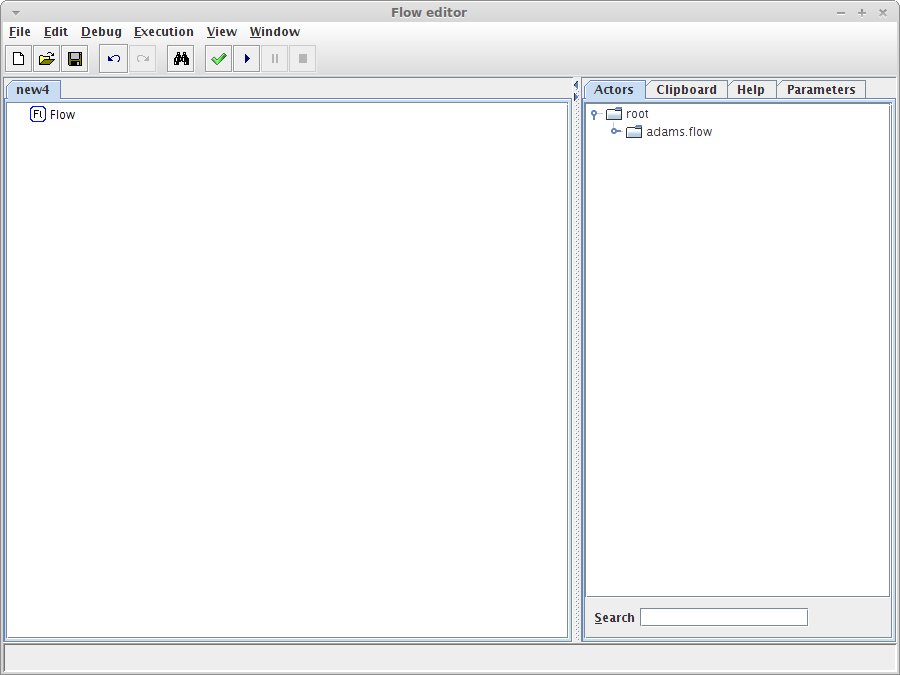
\includegraphics[width=12.0cm]{images/floweditor-new.png}
  \caption{Flow editor with an empty new flow
  (\textit{File $\rightarrow$ New $\rightarrow$ Flow)}}
  \label{floweditor-newflow}
\end{figure}

You can edit as many flows in parallel as you want, e.g., for copy/pasting
actors or other setups between them. Also, you can run them in parallel as well.

\clearpage
\subsection{Hello World}
The first flow \footnote{adams-core-hello\_world1.flow} that we will be setting
up now is very simple: a \textit{source} will output the string \textit{Hello World!} and a \textit{sink} will display
it then. For simplicity, we will just use the right-click menu for adding the
actors to this flow.

Since this is our first flow, we want the display to be as
verbose as possible. Hence make sure to check \textit{Show input/output} from
the \textit{View} menu. This will display what types of inputs and outputs the
various actors accept and/or generate. Once you are familiar with the actors,
you might want to turn this feature off again, especially when the flows become
larger.

First, we need to add the \textit{source} that outputs the string. The
\textit{StringConstants} source can output an arbitrary number of strings that
the user defined. We will use this actor in this simple example.

Select the actor that you want to add an actor before, after or
below. In this case, starting with an empty flow, this is the
\textit{Flow} actor. Now right-click and select \textit{Add beneath\ldots} from
the menu, as shown in Figure \ref{floweditor-helloworld-addactor1}.

\begin{figure}[htb]
  \centering
  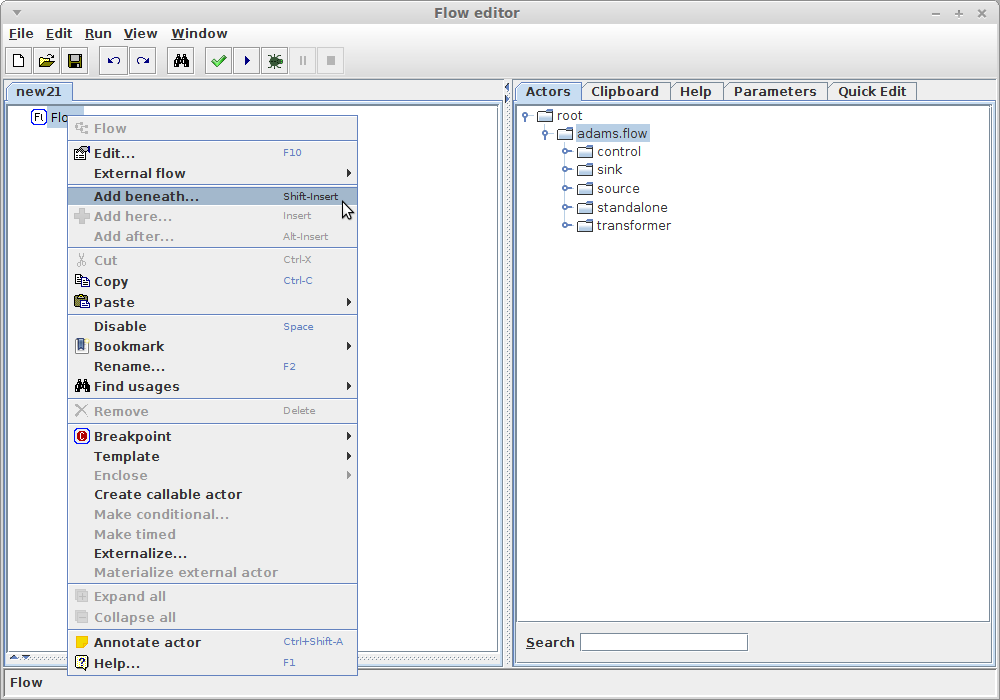
\includegraphics[width=12.0cm]{images/floweditor-helloworld-addactor1.png}
  \caption{Popup menu for adding a new actor}
  \label{floweditor-helloworld-addactor1}
\end{figure}

ADAMS tries to suggest an actor depending on pre-defined rules and the context 
where the actor will get placed. The ones pre-defined by rules will be 
automatically available through the combobox at the top. But due to the large 
amount of actors, quite often you will choose a different one. You can do this 
by simply clicking on the button --
showing an icon of a hierarchical structure - in the top-right corner of the current dialog. A
new popup will be displayed right next to the button (see Figure
\ref{floweditor-helloworld-addactor2}).

\begin{figure}[htb]
  \centering
  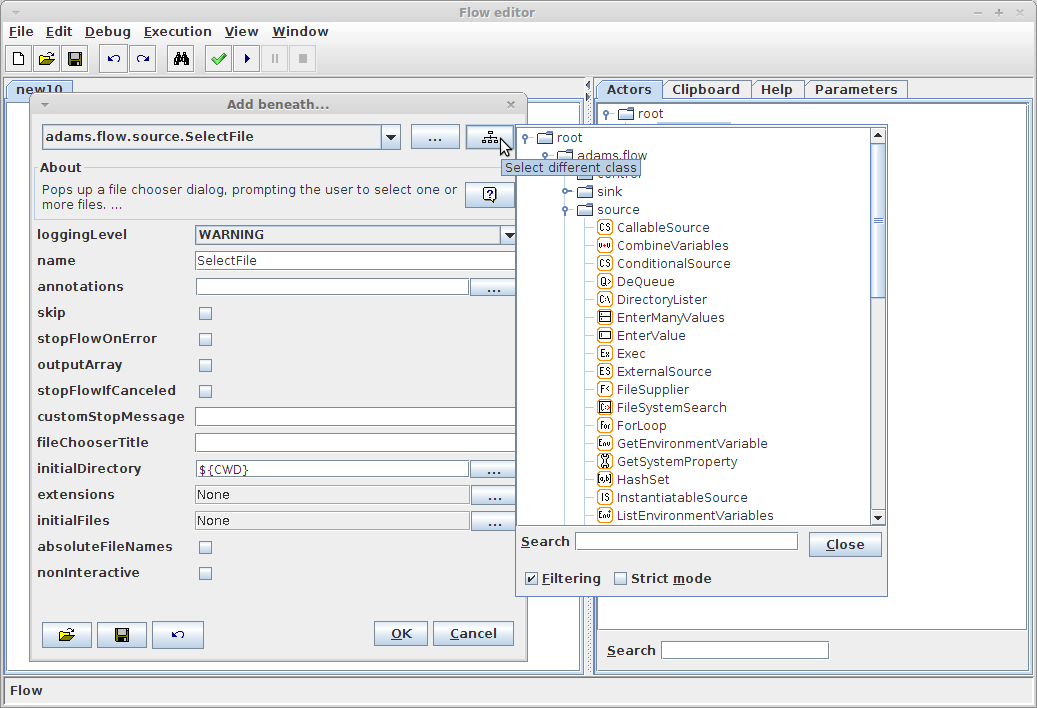
\includegraphics[width=12.0cm]{images/floweditor-helloworld-addactor2.png}
  \caption{Selecting a different actor}
  \label{floweditor-helloworld-addactor2}
\end{figure}

Due to the large amount of available actors \footnote{ADAMS automatically
filters actors that won't fit where you want to place a new actor. Using the
\textit{strict mode}, you can also filter the actors that might only be
compatible, like general purpose ones. Each module can define such rules. Also,
the initial actors that ADAMS suggests are based on pre-defined rules of what
actors are commonly placed in certain situations. If there are more than one
suggestions, a combobox with all the class names is displayed in the
GenericObjectEditor instead of a simple label.}, most of the time it is quicker
to use the search facility of the popup displaying the class tree. Either click
in the search box or use the shortcut \texttt{Alt+S} to jump there. As soon as
you type, the display filters out all the class names that don't match the
entered string. After entering \textit{str} you will see a result similar to
Figure \ref{floweditor-helloworld-addactor3}.

\begin{figure}[htb]
  \centering
  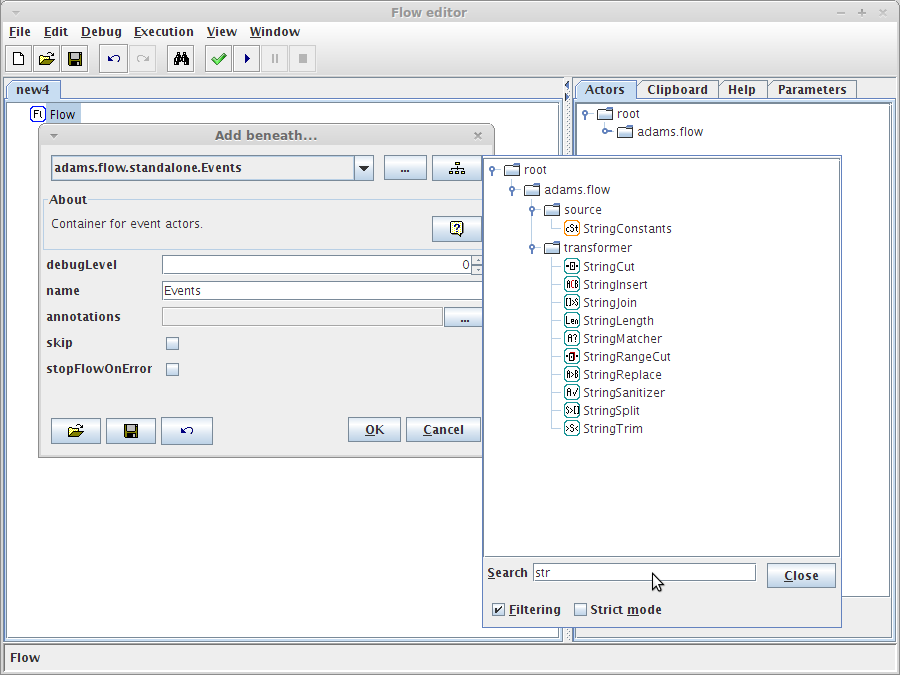
\includegraphics[width=12.0cm]{images/floweditor-helloworld-addactor3.png}
  \caption{Searching for \textit{StringConstants} actor}
  \label{floweditor-helloworld-addactor3}
\end{figure}

Now click on the \textit{StringConstants} actor to select it. The \textit{About}
description only displays some of the information about an actor (normally only
the first sentence of the general description). If you want to know more about
an actor and its options, just click on on the \icon{images/help} button in the
\textit{About} box. For the \textit{StringConstants} actor this opens a dialog
like shown in Figure \ref{floweditor-helloworld-actorhelp}. For quick info on
options, you simply hover with your mouse over one of the options and a tool tip
will come up with the description.

\begin{figure}[htb]
  \centering
  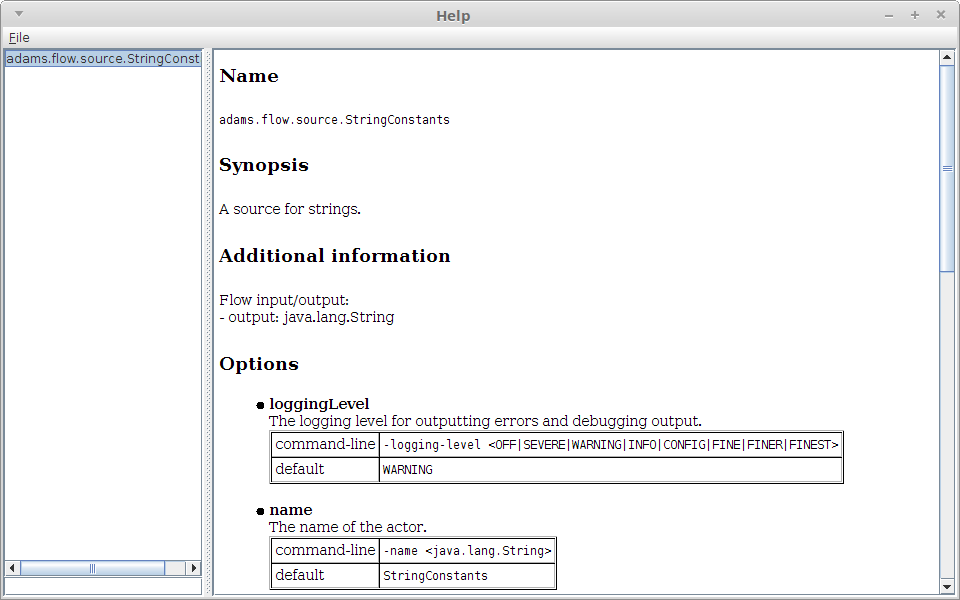
\includegraphics[width=7.0cm]{images/floweditor-helloworld-actorhelp.png}
  \caption{Help dialog for the \textit{StringConstants} actor}
  \label{floweditor-helloworld-actorhelp}
\end{figure}

The \textit{strings} property holds all the user-specified strings that this
source actor will output. In our case, we just want to output
\texttt{Hello World!}. Open up the array editor for the \textit{strings}
property, by clicking on the \texttt{\ldots} button for this property.
In order to enter a string value in this dialog, just click on the
\textit{\ldots} button again and enter the value as shown in Figure
\ref{floweditor-helloworld-addactor4} and click on \textit{OK}.

\begin{figure}[htb]
  \centering
  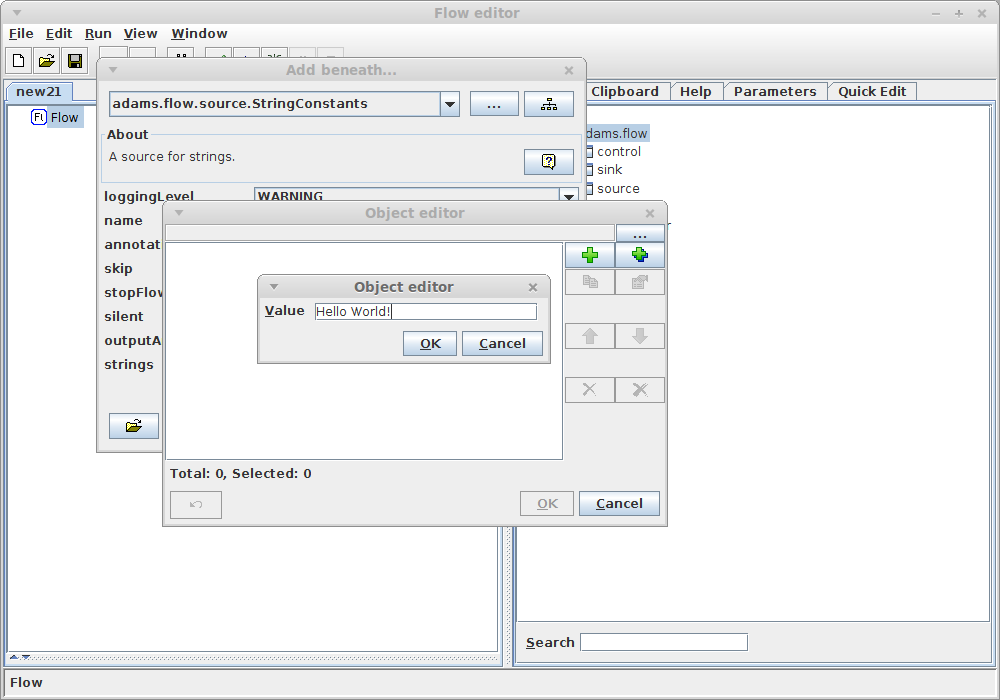
\includegraphics[width=12.0cm]{images/floweditor-helloworld-addactor4.png}
  \caption{Adding the \textit{Hello World!} string}
  \label{floweditor-helloworld-addactor4}
\end{figure}

So far, you have only configured an object (a simple string in this case). Now
you have to add the string object to the list, in order to use it. Just click on
the \icon{images/arrayeditor-add} button on the right-hand side (a
\textit{red} plus sign inidicates a recent change, \textit{green} indicates
that nothing has changed). If you wanted to output more than just one string,
for each of them you would bring up the dialog again, enter the value and add
it to the list. After adding all the necessary items, confirm the dialog by
clicking on the \textit{OK} button.

This finishes our set up of the \textit{StringConstants} actor and you can
confirm the dialog with \textit{OK} button. Figure
\ref{floweditor-helloworld-addactor5} shows the resulting flow.

\begin{figure}[htb]
  \centering
  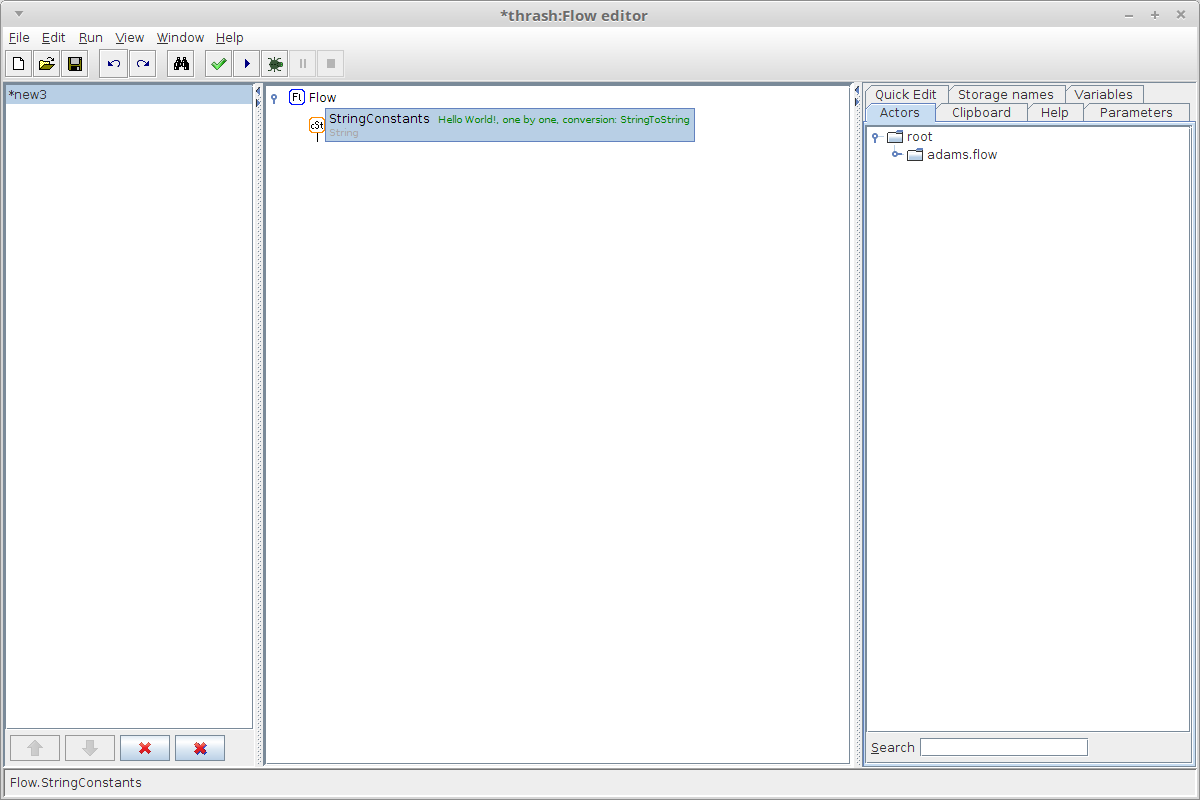
\includegraphics[width=12.0cm]{images/floweditor-helloworld-addactor5.png}
  \caption{Flow after adding the \textit{StringConstants} actor}
  \label{floweditor-helloworld-addactor5}
\end{figure}

The Flow editor offers help also through the tabs on the right hand side. The
\textit{Help} tab (Figure \ref{floweditor-helloworld-actorhelp-tab}) displays
the same information as the aforementioned dialog, but without the need of
opening a new dialog. You merely have to select an actor on the left hand side
in order to display its help screen. The \textit{Parameters} tab is a shortcut
to see all the options of the currently selected actor which differ from the
default options (\ref{floweditor-helloworld-actoroptions}). This can be quite
handy when quickly going through multiple actors, checking their values.
Especially actors with lots of options.

\begin{figure}[htb]
  \centering
  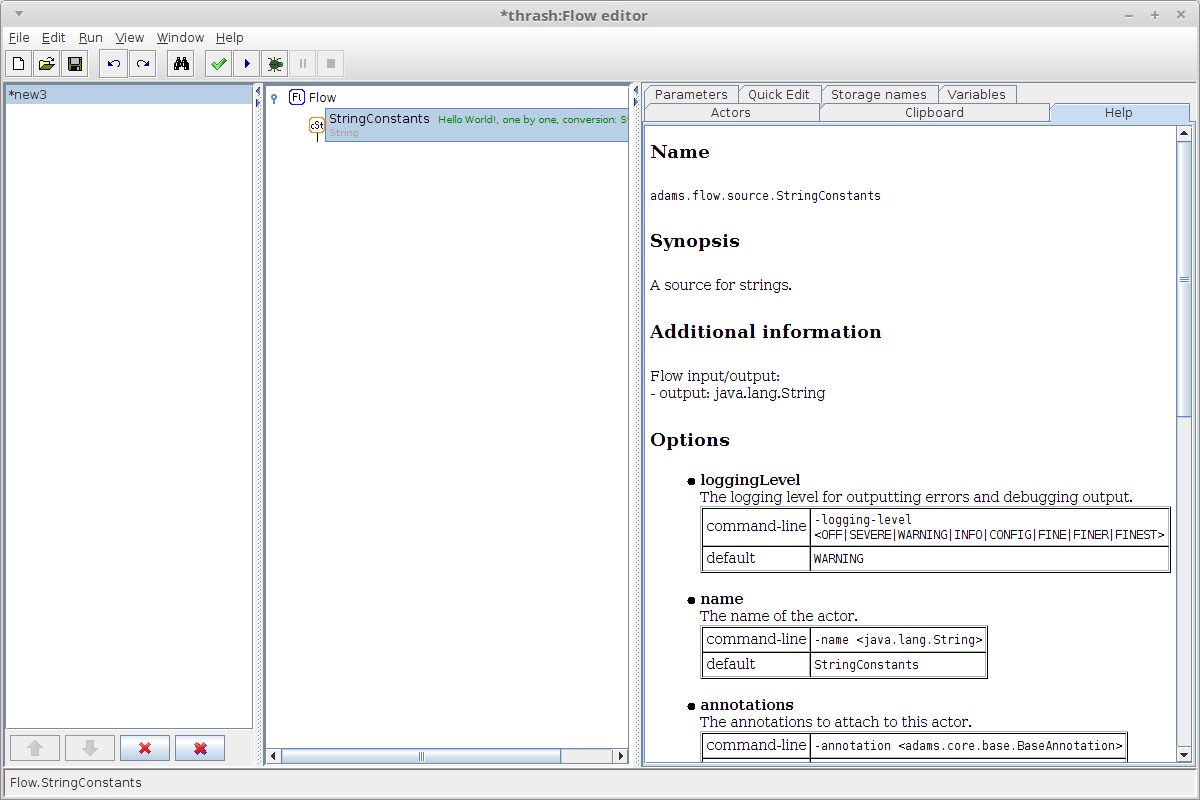
\includegraphics[width=12.0cm]{images/floweditor-helloworld-actorhelp-tab.png}
  \caption{Tab displaying help for the \textit{StringConstants} actor}
  \label{floweditor-helloworld-actorhelp-tab}
\end{figure}

\begin{figure}[htb]
  \centering
  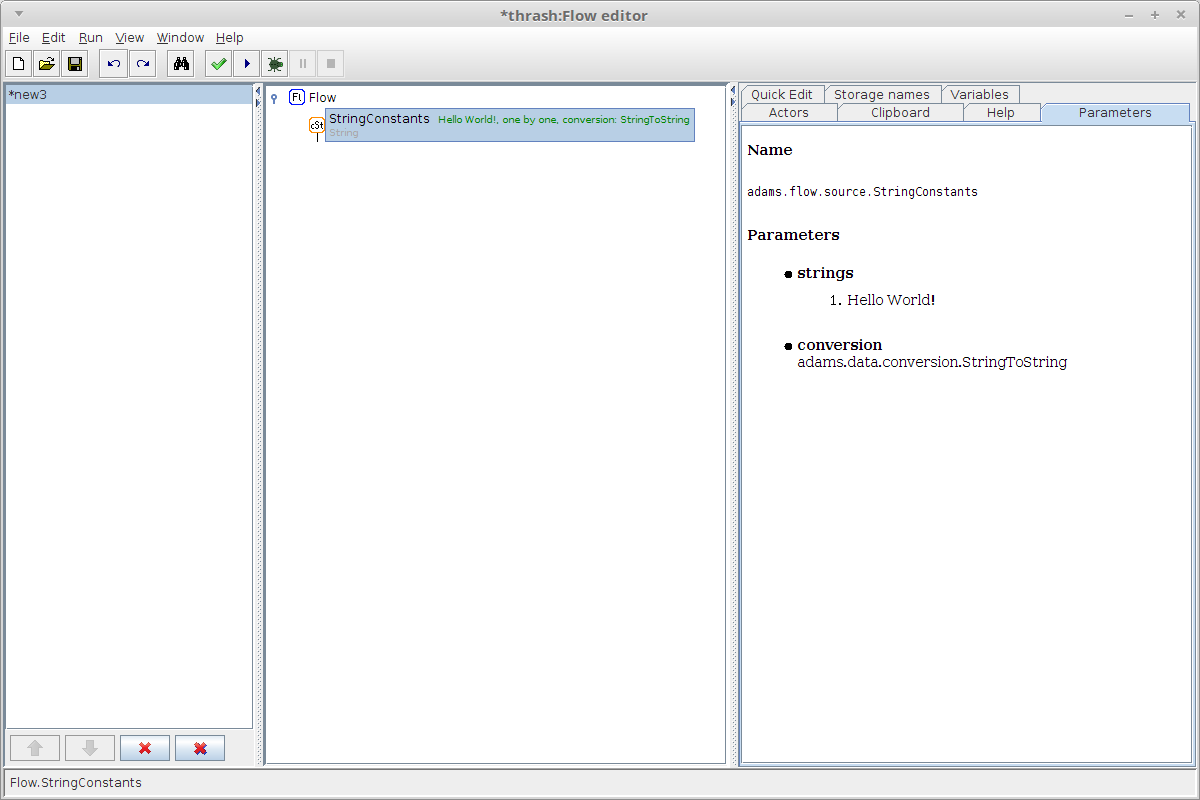
\includegraphics[width=12.0cm]{images/floweditor-helloworld-actoroptions.png}
  \caption{Tab displaying the non-default options for the
  \textit{StringConstants} actor}
  \label{floweditor-helloworld-actoroptions}
\end{figure}

For our simple \textit{Hello World} example, we don't need an data processing
using \textit{transformer} actors, only a \textit{sink} that will display our
data. The \textit{Display} actor can be used for displaying textual data. This
actor adds the string representation of each token that it receives as a new
line in its text area.

For adding the \textit{Display} actor, right-click on the previously added
\textit{StringConstants} actor and select \textit{Add after\ldots} as shown in
Figure \ref{floweditor-helloworld-addactor6}.

\begin{figure}[htb]
  \centering
  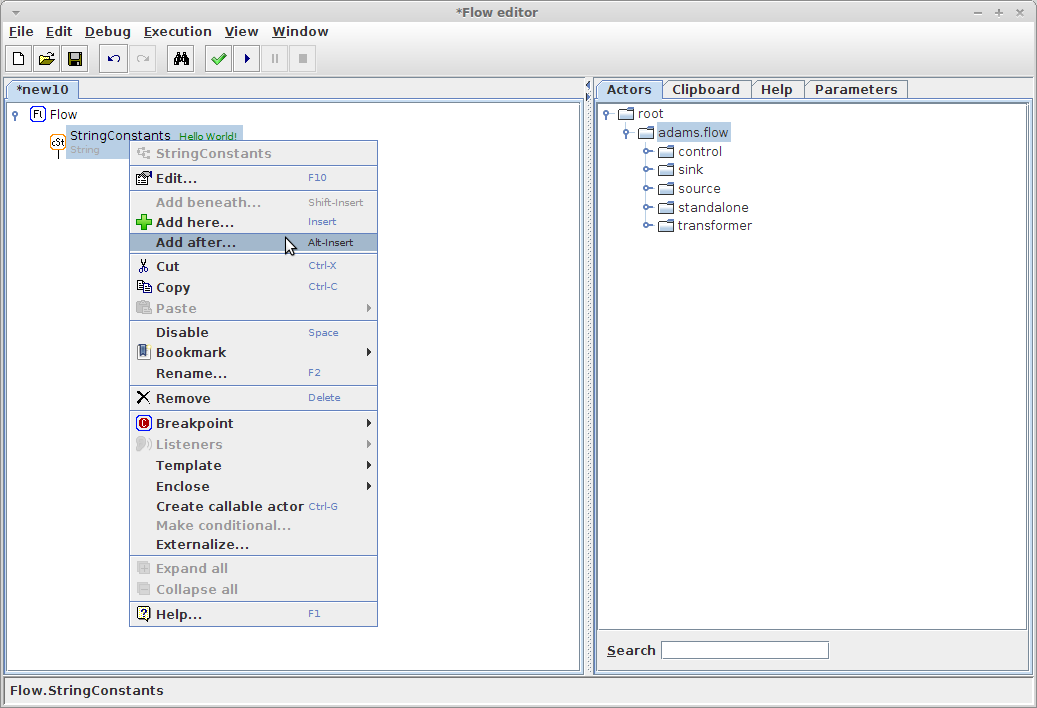
\includegraphics[width=12.0cm]{images/floweditor-helloworld-addactor6.png}
  \caption{Adding another actor \textit{after} the current one}
  \label{floweditor-helloworld-addactor6}
\end{figure}

Once again, bring up the class tree dialog with all the actors by clicking on
the button in the top-right corner of the actor dialog. This time, you have to
search for \textit{Display}. As soon as you have entered \textit{dis} you will
see the dialog showing a filtered class tree as shown in Figure
\ref{floweditor-helloworld-addactor7}.

\begin{figure}[htb]
  \centering
  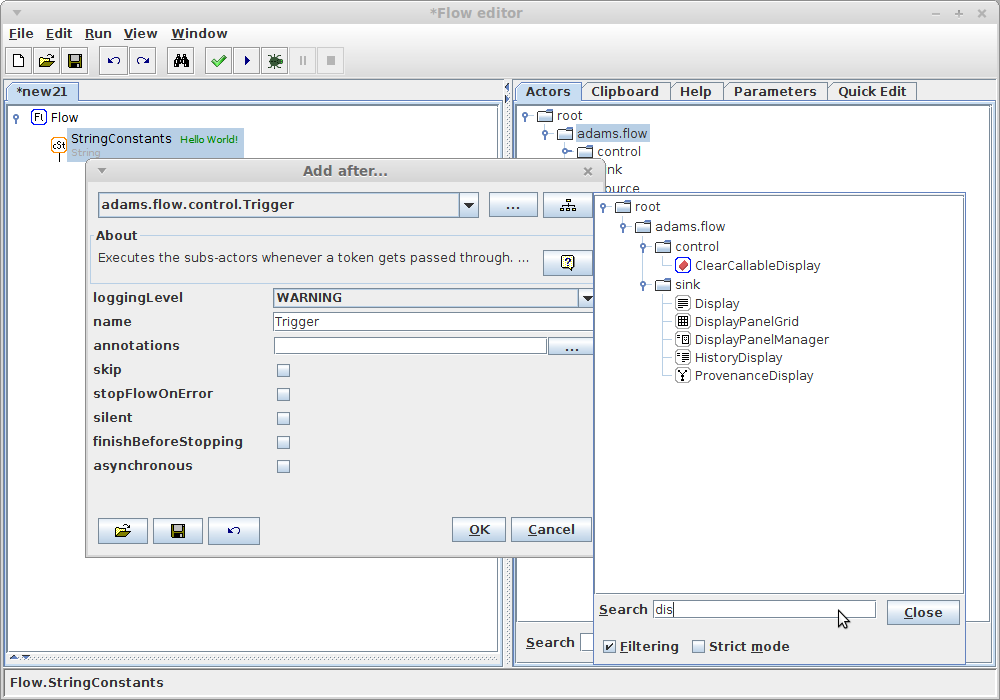
\includegraphics[width=12.0cm]{images/floweditor-helloworld-addactor7.png}
  \caption{Searching for the \textit{Display} actor}
  \label{floweditor-helloworld-addactor7}
\end{figure}

Select the \textit{Display} actor, just like you did with the
\textit{StringConstants} actor. Since we don't have to configure anything for
this actor -- it merely displays our data -- you can just confirm it by clicking
on \textit{OK} again.

This completes our flow for this simple example and you can save the set up. The
final flow is shown in Figure \ref{floweditor-helloworld-flow}.

\begin{figure}[htb]
  \centering
  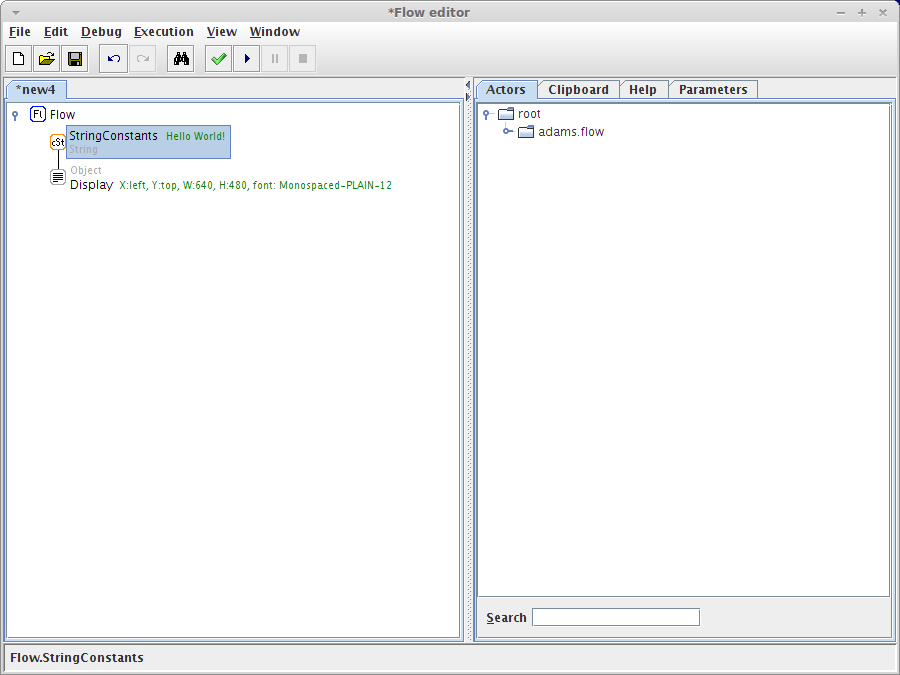
\includegraphics[width=12.0cm]{images/floweditor-helloworld-flow.png}
  \caption{The complete \textit{Hello World} flow}
  \label{floweditor-helloworld-flow}
\end{figure}

With the flow finished, we can now execute it. In the Flow editor menu, select
\textit{Run $\rightarrow$ Run}. Or use the keyboard shortcut
\texttt{Ctrl+R}. Figure \ref{floweditor-helloworld-output} shows the result
output.

\begin{figure}[htb]
  \centering
  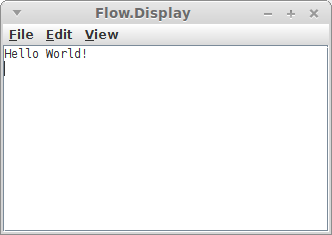
\includegraphics[width=6.0cm]{images/floweditor-helloworld-output.png}
  \caption{The output of \textit{Hello World} flow}
  \label{floweditor-helloworld-output}
\end{figure}

Well done, your first flow is set up and produces output!

\clearpage
\subsection{Processing data}
Of course, for simply outputting some string, you don't need a workflow engine.
The idea of a workflow is to be able to define all steps for
processing the data, not just simply loading and displaying it.

The following steps extend our flow \footnote{adams-core-hello\_world2.flow}
with some string processing: first, turning the initial string into upper case
and, second, appending some text at the
end.

Basic string processing can be performed with the \textit{Convert} transformer.
This actor allows you to choose a conversion class that performs the actual
transformation.

Since our flow only consists of a source and a sink, we need to insert the
transformer in between the two of them. In our example we right-click on the
sink actor and then choose \textit{Add here\ldots}, as you can see in Figure
\ref{floweditor-helloworld-processdata1}. But you can also right-click on the
source and then choose \textit{Add after\ldots}.

The \textit{Add here\ldots} action always moves the actor on which you clicked
one further down and adds the chosen one at the current position. The
\textit{Add after\ldots}, adds the chosen actor after the one that you clicked
on.

\begin{figure}[htb]
  \centering
  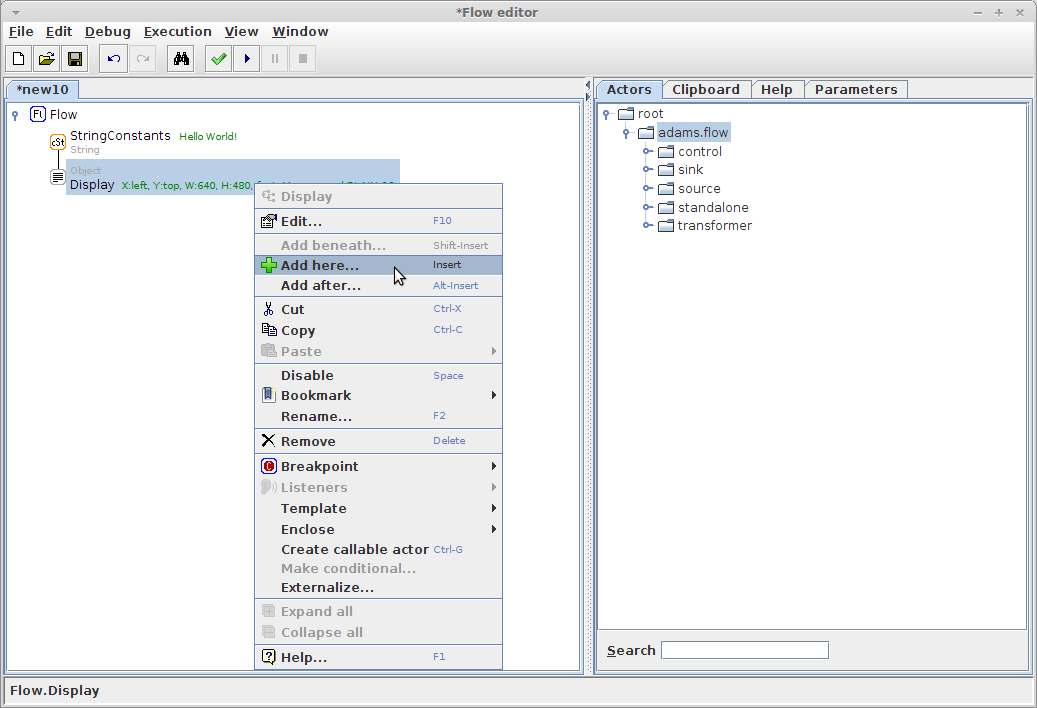
\includegraphics[width=12.0cm]{images/floweditor-helloworld-processdata1.png}
  \caption{Adding an additional actor}
  \label{floweditor-helloworld-processdata1}
\end{figure}

Now choose the \textit{Convert} transformer from the class tree, e.g., by
searching for it, as displayed in Figure
\ref{floweditor-helloworld-processdata2}.

\begin{figure}[htb]
  \centering
  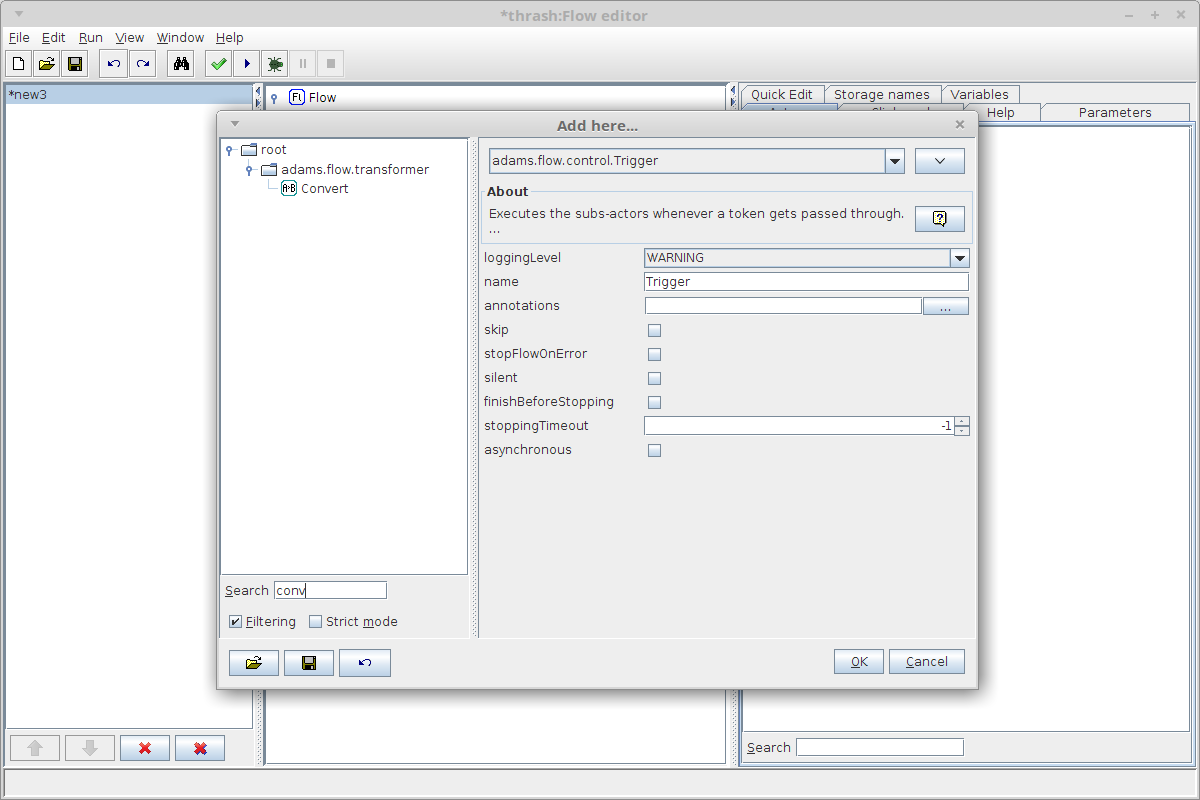
\includegraphics[width=12.0cm]{images/floweditor-helloworld-processdata2.png}
  \caption{Adding the \textit{Convert} transformer}
  \label{floweditor-helloworld-processdata2}
\end{figure}

Change the type of \textit{conversion} to \textit{UpperCase} (Figure
\ref{floweditor-helloworld-processdata3}).

\begin{figure}[htb]
  \centering
  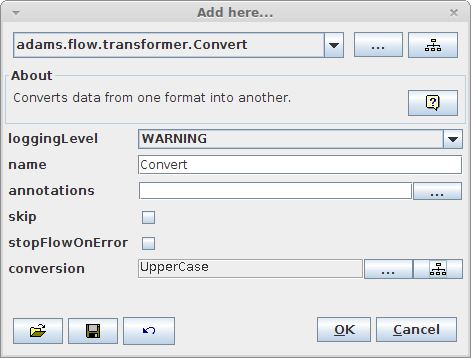
\includegraphics[width=6.0cm]{images/floweditor-helloworld-processdata3.png}
  \caption{Configuring the \textit{Convert} transformer}
  \label{floweditor-helloworld-processdata3}
\end{figure}

The flow should now look like Figure \ref{floweditor-helloworld-processdata4}
and, when you execute it, produce output as shown in Figure
\ref{floweditor-helloworld-processdata5}. This concludes our first
string processing step.

\begin{figure}[htb]
  \centering
  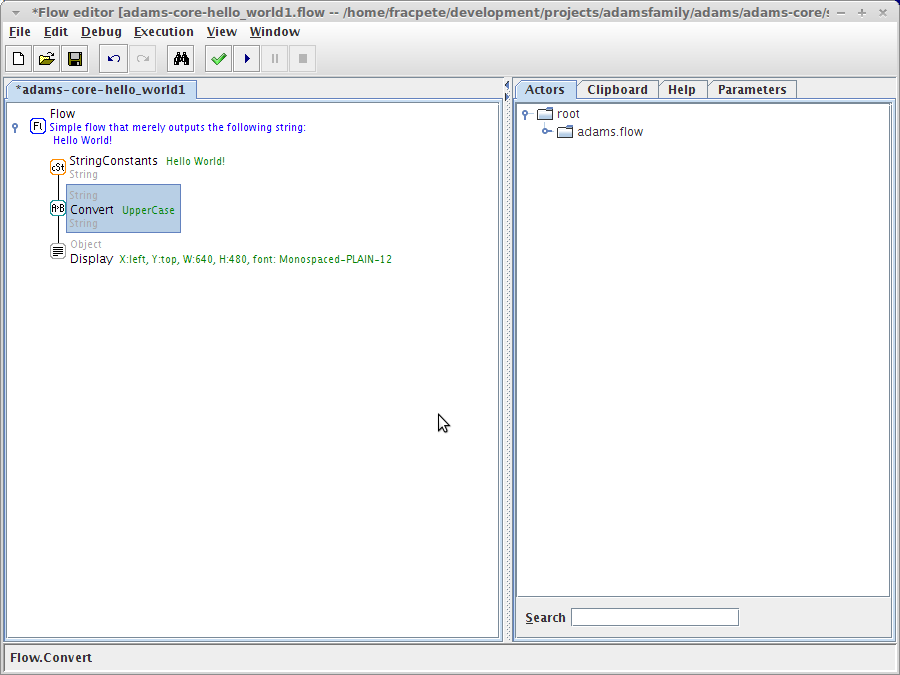
\includegraphics[width=12.0cm]{images/floweditor-helloworld-processdata4.png}
  \caption{Extended \textit{Hello World} flow}
  \label{floweditor-helloworld-processdata4}
\end{figure}

\begin{figure}[htb]
  \centering
  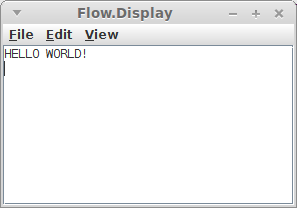
\includegraphics[width=5.0cm]{images/floweditor-helloworld-processdata5.png}
  \caption{Output of the extended \textit{Hello World} flow}
  \label{floweditor-helloworld-processdata5}
\end{figure}

The second string processing step \footnote{adams-core-hello\_world3.flow}
requires adding a custom string at the end of the actor outputting \textit{HELLO
WORLD!}. We can achieve this by using the \textit{StringReplace} actor, which allows us to perform string replacements
using regular expressions \footnote{For more information see
\url{http://en.wikipedia.org/wiki/Regular_expressions}{}.}. In this case, the
replacement is very simple: replacing the end of the string (``\$'') with the
string that we want to append `` How are you today!'' (see Figure
\ref{floweditor-helloworld-processdata6}).

\begin{figure}[htb]
  \centering
  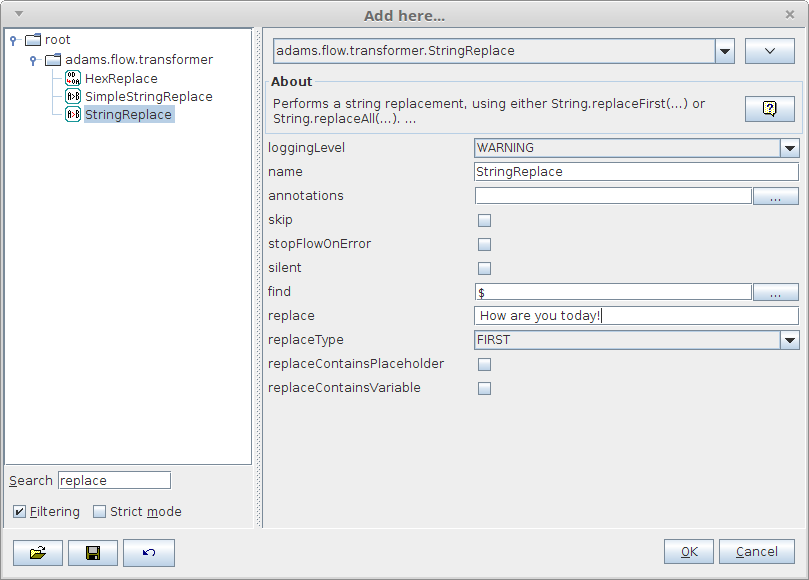
\includegraphics[width=6.0cm]{images/floweditor-helloworld-processdata6.png}
  \caption{Customizing the \textit{StringReplace} transformer}
  \label{floweditor-helloworld-processdata6}
\end{figure}

In a lot of cases, regular expressions can be overkill for manipulating strings.
E.g., when prepending or appending a string. In such simple cases, you also
just use the simpler \textit{StringInsert} transformer.

Executing the flow now will produce output as seen in Figure
\ref{floweditor-helloworld-processdata7}.

\begin{figure}[htb]
  \centering
  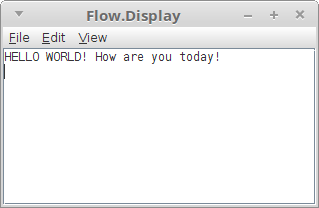
\includegraphics[width=6.0cm]{images/floweditor-helloworld-processdata7.png}
  \caption{Output of further extended \textit{Hello World} flow}
  \label{floweditor-helloworld-processdata7}
\end{figure}

\clearpage
\subsection{Control actors}
So far, we have only covered linear execution of actors, where one actor is
executed after the other. For this linear approach, a workflow still seems like
overkill. In the following sections we will introduced \textit{control actors},
which \textit{control} the flow of data within the flow in some way or another.

\subsubsection{Have some \textit{Tee}}
The \textit{Tee} actor, like the Unix/Linux \textit{tee} command, allows you to
fork off the data that is being passed through and re-use it for something else.
For example for debugging purposes, when you need to investigate the data
generation at various stages throughout the flow.

In the following example \footnote{adams-core-hello\_world4.flow} we will use
the \textit{Tee} actor to document the various stages of transformation that the \textit{Hello World!} string goes
through. Three \textit{Tee} actors will be placed in the flow: one right after
the \textit{StringConstants} source, the next after the \textit{Convert}
transformer, and the last after the \textit{StringReplace} transformer.
Each time, a \textit{DumpFile} sink will be added beneath the \textit{Tee}
actor, pointing to the same log file. In our example, we are using
\texttt{/tmp/out.txt} - adjust it to fit your system. By default, the
\textit{DumpFile} actor overwrites the content of the file if it already exists.
This is fine for the first occurrence, but for the second and third one we need
to check the \textit{append} option. Otherwise we will lose the previous
transformation steps. The fully expanded flow is shown in Figure
\ref{floweditor-helloworld-tee_flow}.
\begin{figure}[htb]
  \centering
  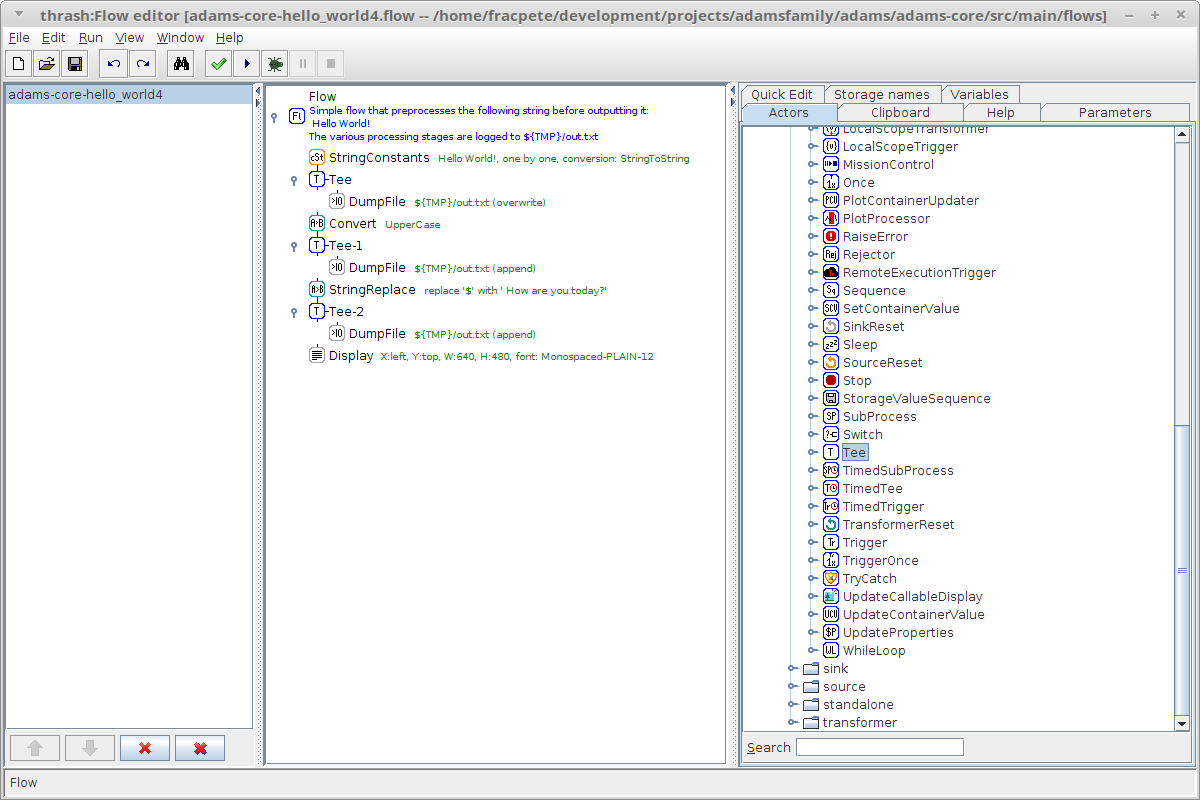
\includegraphics[width=12.0cm]{images/floweditor-helloworld-tee_flow.png}
  \caption{The \textit{Hello World} flow with \textit{Tee} actors.}
  \label{floweditor-helloworld-tee_flow}
\end{figure}
Figure \ref{floweditor-helloworld-tee_logfile} shows the generated log file in a
text editor.
\begin{figure}[htb]
  \centering
  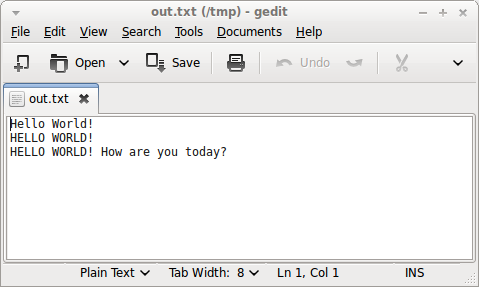
\includegraphics[width=6.0cm]{images/floweditor-helloworld-tee_logfile.png}
  \caption{The log file generated by the \textit{Tee} actors.}
  \label{floweditor-helloworld-tee_logfile}
\end{figure}

The \textit{ConditionalTee} control actor is an extended version of the simple
\textit{Tee} actor. This actor only tees off the token if its boolean condition
returns \textit{true}. For instance, using the \textit{Counting} condition, this
actor will keep track of the number of data tokens passing through. This allows
you to specify rules for when to fork off the data tokens.
For instance, you can configure it that only every third token gets forked off,
starting with the 100th one and stopping with the 200th token (to be precise,
the first token output is the 102nd and the last one the 198th one). See Figure
\ref{floweditor-conditionaltee} for an example of this set up.
\begin{figure}[htb]
  \centering
  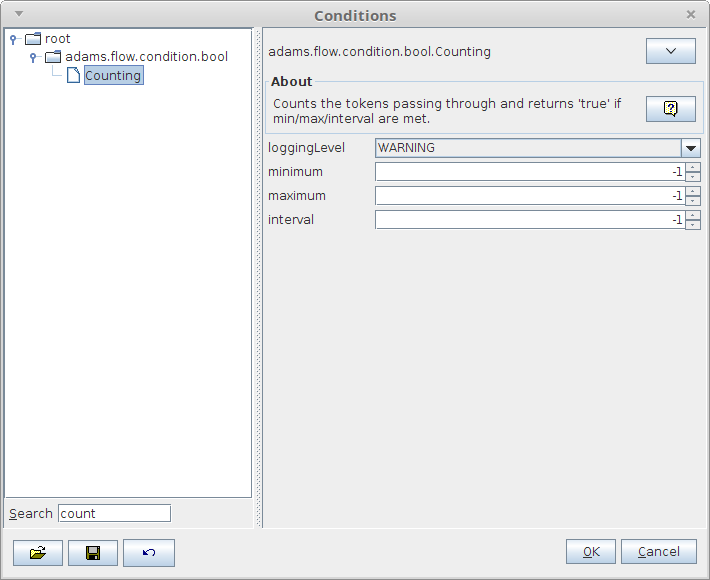
\includegraphics[width=5.0cm]{images/floweditor-conditionaltee.png}
  \caption{A customized \textit{ConditionalTee} actor.}
  \label{floweditor-conditionaltee}
\end{figure}

A close cousin to the \textit{ConditionalTee} actor is the \textit{Count} actor.
This actor offers the same conditions as the \textit{ConditionalTee} for the
tee output, but instead of forking off the current data token, it forks off the
number of tokens it has encountered so far. Very useful when trying to keep
track of how much data has been processed.

\subsubsection{Pull the \textit{Trigger}}
The \textit{Trigger} control actor is used to initiate the execution of a
sub-flow. In contrast to the \textit{Tee} actor, the \textit{Trigger} does not
fork off any token, it merely triggers the execution of the actors defined below
it. Since no data is being forked off, a source actor is required in the
sub-flow to kick off the other actors. Using a trigger
\footnote{adams-core-hello\_world5.flow} we can inject another string into the
log file that was generated in the previous example, as Figure \ref{floweditor-helloworld-trigger_flow}.
\begin{figure}[htb]
  \centering
  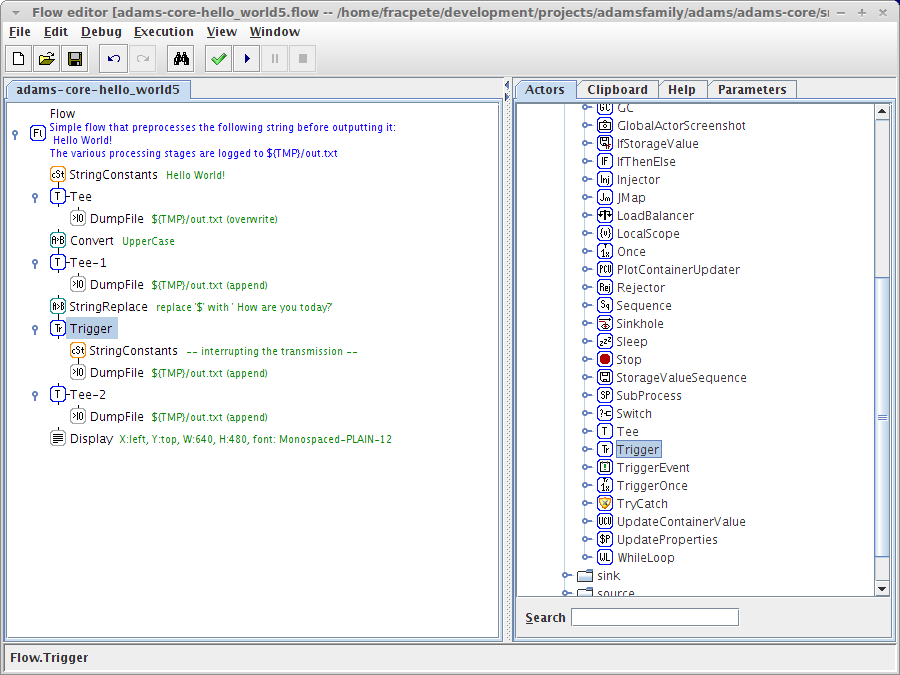
\includegraphics[width=12.0cm]{images/floweditor-helloworld-trigger_flow.png}
  \caption{The \textit{Hello World} flow with an additional \textit{Trigger}
  actor.}
  \label{floweditor-helloworld-trigger_flow}
\end{figure}
Figure \ref{floweditor-helloworld-trigger_logfile} shows the modified
log file in a text editor.
\begin{figure}[htb]
  \centering
  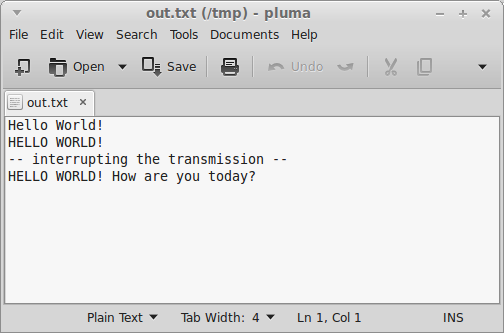
\includegraphics[width=6.0cm]{images/floweditor-helloworld-trigger_logfile.png}
  \caption{The modified log file generated with the additional \textit{Trigger}
  actor.}
  \label{floweditor-helloworld-trigger_logfile}
\end{figure}
The \textit{Trigger} actor is also the only other control actor, besides the
\textit{Flow} control actor, that allows \textit{standalone} actors to be added
to it.

A variant of the \textit{Trigger} actor is the \textit{ConditionalTrigger}
actor. This actor only executes the sub-flow if its boolean condition returns
\textit{true}. \textit{TriggerOnce}, another variant, triggers the sub-flow 
exactly once, useful for initializations.

\subsubsection{Branching -- or how to grow your flow}
So far, we have only processed data in a sequential way. The \textit{Branch}
actor allows the parallel processing of the same token. Each sub-branch receives
the same token for further processing. In Figure
\ref{floweditor-helloworld-branch_flow}, we re-use our simple example,
outputting \textit{Hello World} in parallel, displaying the results in two
different \textit{Display} actors \footnote{adams-core-hello\_world6.flow}. The
second sub-branch processes the original string further. As you can see from this example, as soon as you have more than
one actor, you need to encapsulate the actors in a \textit{Sequence} control
actor.
\begin{figure}[htb]
  \centering
  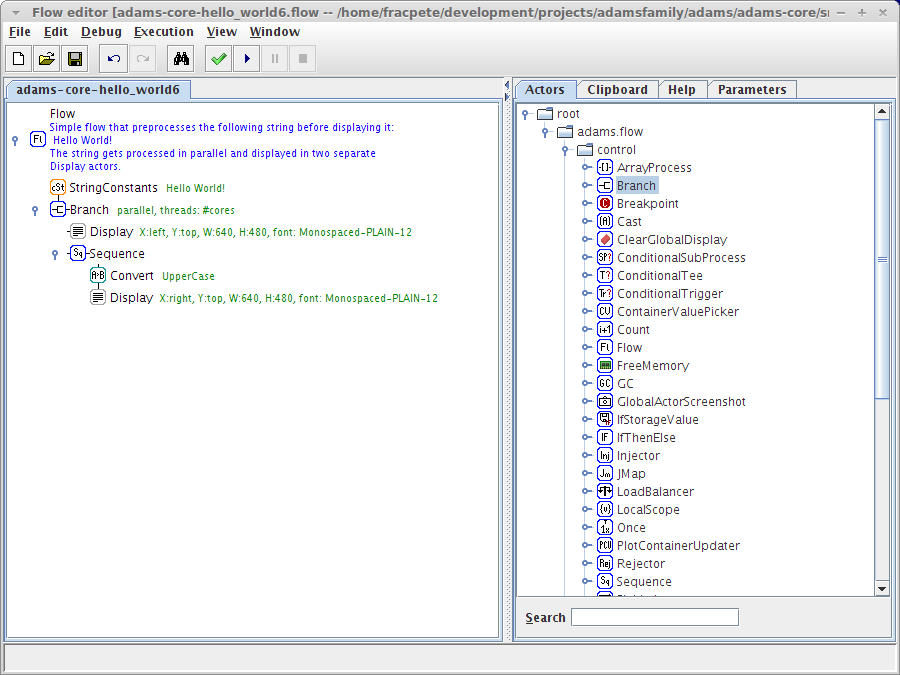
\includegraphics[width=12.0cm]{images/floweditor-helloworld-branch_flow.png}
  \caption{The \textit{Hello World} flow using a \textit{Branch} actor.}
  \label{floweditor-helloworld-branch_flow}
\end{figure}
The default setting of the \textit{Branch} actor is to process the branches in
separate threads, taking the maximum number of cores/CPUs of the underlying
architecture into account. But it is also possible to enforce a sequential
execution of the sub-branches, by setting the \textit{number of threads} to
\textbf{0}. There are two reasons fro this:
\begin{enumerate}
  \item \textit{Resources} -- If the branch is located deeper in the flow with
  other parallel execution happening, spawning too many threads can slow down
  the system more than it could help in the optimal case. In such a scenario, it
  is advised to turn off parallel execution.
  \item \textit{Ordering} -- In certain cases, the same data needs to be
  processed several times, but the order of the in which this occurs is
  important. For instance, an integer token could be used to create a
  sub-directory in which to store the value of the integer token in a file.
  These two sub-branches need to get executed one after the other, of course.
\end{enumerate}

\subsubsection{Further control actors}
The \textit{Branch}, \textit{Tee} and \textit{Trigger} control actors are just
some of the more commonly used ones. ADAMS comes already with a wide variety of
control actors. In the following a short introduction to the others:
\begin{tight_itemize}
	\item \textit{ArrayGenerate} -- generates an array of the output
	generated by its sub-actors, using the same input token.
	\item \textit{ArrayProcess} -- instead of unraveling an array with
	\textit{ArrayToSequence} and then packaging again with
	\textit{SequenceToArray}, this actor allows to perform an arbitrary number of
	sub-steps on an incoming array.
	\item \textit{Breakpoint} -- Used for debugging a flow. See
	\ref{debugging_flow} for more details.
	\item \textit{ClearCallableDisplay} -- Can be used to clear callable
	graphical actors, e.g., a \textit{SequencePlotter}. See \ref{callable_actors} for
	more information on callable actors.
	\item \textit{ConditionalTee} -- Basically like the \textit{Tee} actor, but it
	allows you to impose constraints on when to tee off the tokens.
	\item \textit{ContainerValuePicker} -- Since ADAMS only allows \textit{1-to-1}
	and \textit{1-to-n} connections, multiple outputs are usually packaged in
	\textit{containers}. The values in the container can be accessed by their name
	(check the specific actor's documentation on what the names are) using this
	actor.
	\item \textit{Continue} -- Does not pass on tokens if the specified boolean
	expression evaluates to \textit{true}, i.e., acts like the ``continue'' 
	control statement.
	\item \textit{Count} -- In contrast to \textit{ConditionalTee}, this actor tees
	off the number of tokens it has encountered so far. Useful for lengthy
	processes, if you want to keep track of how many tokens you have processed so
	far.
	\item \textit{DesktopScreenshot} -- allows you to take a screenshot
	of the complete desktop.
	\item \textit{FreeMemory} -- Invokes the parent to wrap up all its
	sub-actors, effectively freeing up memory. Useful if branches of a
	many-branched \textit{Branch} actor only get executed once, but still keep
	their state and hog memory.
	\item \textit{GC} -- For explicitly executing the Java garbage collection.
	\item \textit{CallableActorScreenshot} -- For taking screenshots of a callable
	(graphical) actor, whenever a token passes through this control actor.
	See \ref{callable_actors} for more information on callable actors.
	\item \textit{IfStorageValue} -- An \textit{if-then-else} source that executes
	the \textit{then} branch if the specified storage value exists. Otherwise it
	executes the \textit{else} branch, which needs to have a source actor for
	generating actual data.
	\item \textit{IfThenElse} -- A control statement, which evaluates a boolean
	condition in order to decide in which branch to pass on the incoming token.
	\item \textit{Injector} -- Allows you to inject tokens into the stream of
	tokens.
	\item \textit{InputOutputListener} -- Enables forwarding incoming tokens
	and tokens generated by sub-flow to callable actors.
	\item \textit{Inspect} -- A more specialized actor for \textit{visualizing} data
	that is passing through the flow, interactively or not.
	\item \textit{JMap} -- If available, i.e., using a JDK instead of JRE, you can
	output information on what objects are currently present in the JVM. Useful for
	hunting down memory leaks.
	\item \textit{LoadBalancer} -- Spawns off threads for incoming tokens to
	process the tokens independently in the sub-flow defined below this actor.
	\item \textit{LocalScopeTransformer} -- Provides ``local'' variables and internal
	storage; useful when things run in parallel.
	\item \textit{LocalScopeTrigger} -- Provides ``local'' variables and internal
	storage; useful when things run in parallel.
	\item \textit{Once} -- A tee actor that only tees off the first token it
	encounters. A simplified \textit{ConditionalTee} so to speak.
	\item \textit{MissionControl} -- shows a minimalistic control panel
	for pausing, resuming and stopping the flow.
	\item \textit{PlotContainerUpdater} -- Allows one to update the \textit{name},
	\textit{x} or \textit{y} value stored in a plot container. Useful for
	post-processing of plot containers, e.g., for scaling.
	\item \textit{RaiseError} -- Raises an error if its condition evaluates to
	\textit{true} using the specified error message (see \textit{TryCatch}).
	\item \textit{Rejector} -- Rejects tokens container data containers that have
	error messages attached.
	\item \textit{Sequence} -- Allows to specify multiple actors that get exectued
	one after the other, with the output of one actor being the input of the next.
	\item \textit{ConditionalSequence} -- Basically like the \textit{Sequence}
	actor, but it allows you to impose constraints on when to process the tokens
	with actors defined in the sequence.
	\item \textit{SetContainerValue} -- Updates a single value of the container
	passing through, using either data obtained from storage or a callable actor.
	\item \textit{SinkReset} -- resets all its sub-actors in case the monitored
	variable changed value.
	\item \textit{Sleep} -- Suspends the flow execution for the specified number of
	milliseconds.
	\item \textit{SourceReset} -- resets all its sub-actors in case the monitored
	variable changed value.
	\item \textit{Stop} -- If executed, stops the flow execution.
	\item \textit{StorageValueSequence} -- For processing the same storage value
	multiple times in Triggers and/or Tees, but still outputting and forwarding
	it in the flow.
	\item \textit{SubProcess} -- Like \textit{Sequence} actor, but the last actor
	definitely has to produce output, i.e., cannot be a \textit{sink}.
	\item \textit{ConditionalSubProcess} -- Basically like the \textit{SubProcess}
	actor, but it allows you to impose constraints on when to process the tokens
	with actors defined in the sub-process.
	\item \textit{Switch} -- Allows an arbitrary number of branches, which get
	forwarded the token if the corresponding condition evaluates to \textit{true}.
	\item \textit{TransformerReset} -- resets all its sub-actors in case the monitored
	variable changed value.
	\item \textit{TryCatch} -- Allows you to protect a sub-flow in a ``try''
	block. If the execution fails for some reason the ``catch'' sub-flow gets
	executed to ensure that flow execution continues (see \textit{RaiseError}).
	\item \textit{UpdateContainerValue} -- Applies all defined sub-actors to the
	specified element of the container that is passing through.
	\item \textit{UpdateProperties} -- Updates multiple properties of an actor
	wrapping a non-ADAMS object, using current variable values.
	\item \textit{WhileLoop} -- Executes the sub-flow as long as the boolean
	condition evaluates to \textit{true}.
\end{tight_itemize}

\subsection{Protecting sub-flows}
By default, ADAMS tries to stop the flow execution as fast as possible. However,
this behavior might not be desired in case of mission critical steps that should
never get interrupted. For instance, when reading (and in the same step, removing)
data from the database, that the output of said data on disk should get 
interrupted. 

In order to allow the user to protect the execution of certain 
sub-flows, a fair amount of actors offer a flag for \textit{atomic execution}.
This flag is called \textit{finishBeforeStopping} in the option dialog. When 
enabled, this actor will wait with stopping its sub-actors until the sub-actors
have finished processing all their data. Actors that support this, are for 
example, \textit{Sequence}, \textit{Branch}, \textit{Tee}, \textit{Trigger} 
(and derived classes).

Be careful how and where you use this flag, as it can have undesired 
side-effects: if you enable this flag in the \textit{Flow} control actor, then 
the flow cannot be stopped before all processing has finished.

\newpage
\section{Running flows}
\label{running_flows}
Executing flows from the \textit{Flow editor} is just one of the options of
how to execute a flow. Unless you want the ability to edit the flow, you could 
use one of the following options.

\subsection{Flow runner - GUI}
The \textit{Flow runner} is an interface to execute flows without the user
being able to modify them. This interface is used for merely executing flow.
This can be useful for users that only \textit{run} flows, but never modify
them. Depending on the flow, the user is still able to influence its 
execution. The Flow runner interface analyzes the flow and displays the 
topmost \texttt{SetVariable} standalones as parameters that the user then
can modify. Figure \ref{floweditor-mandelbrot} shows the flow in the editor
interface and Figure \ref{flowrunner-mandelbrot} in the runner interface.
Annotations that are attached to the \texttt{SetVariable} actors are available
as help through a button next to the edit field with the variable value.

\begin{figure}[htb]
  \centering
  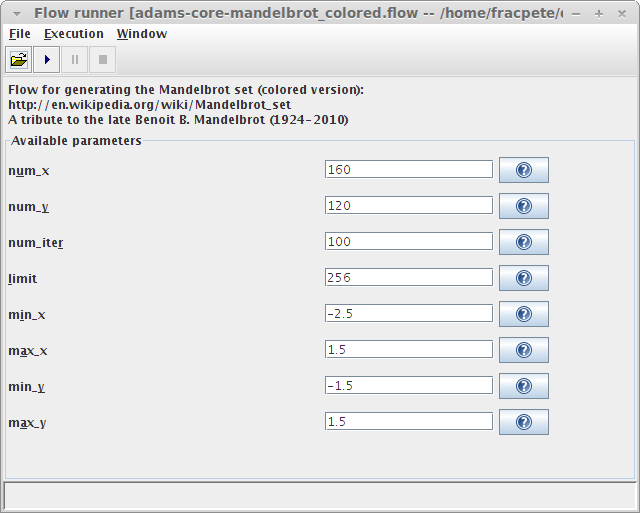
\includegraphics[width=12.0cm]{images/flowrunner-mandelbrot.png}
  \caption{Flow runner interface with a flow for generating the Mandelbrot set.}
  \label{flowrunner-mandelbrot}
\end{figure}

\begin{figure}[htb]
  \centering
  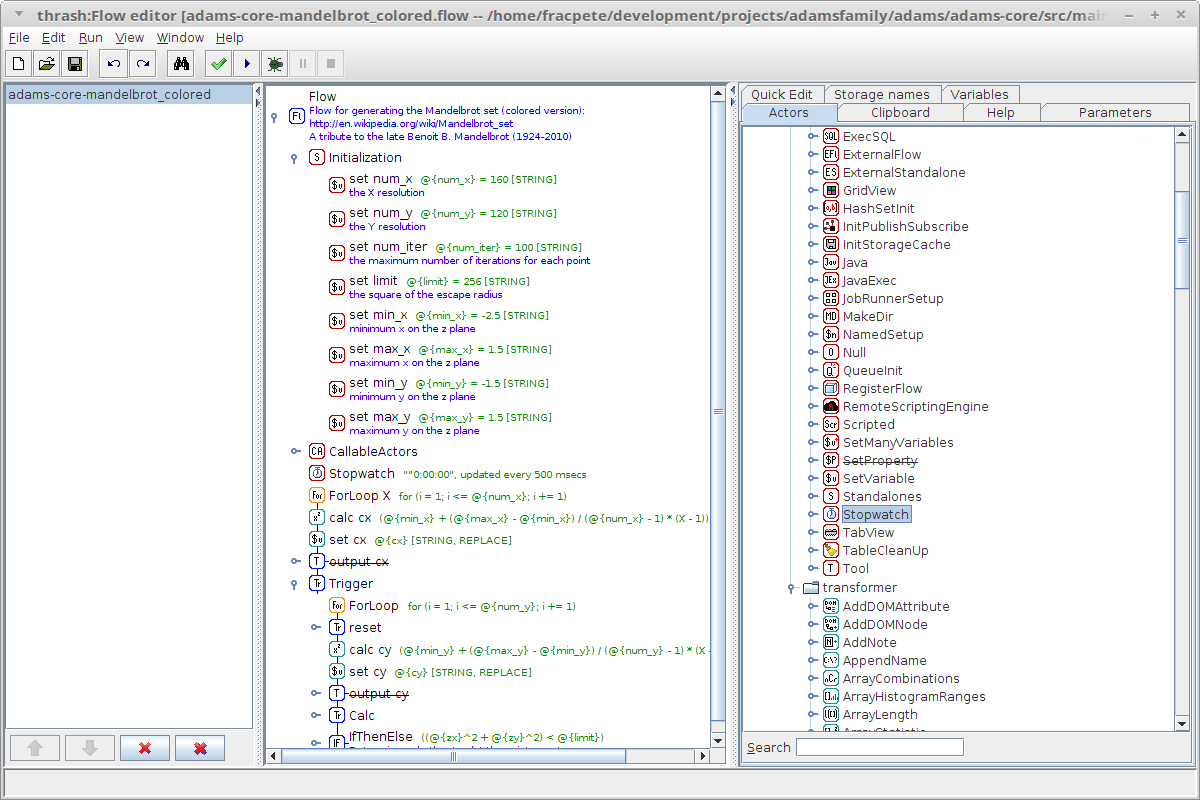
\includegraphics[width=12.0cm]{images/floweditor-mandelbrot.png}
  \caption{Flow editor interface with a flow for generating the Mandelbrot set.}
  \label{floweditor-mandelbrot}
\end{figure}

\subsection{Flow runner - command-line}
The ability to run flows on a server, in a headless environment, was one the
requirements when desinging ADAMS. This can be either for data processing
flows that poll directories or databases or scheduled executions. The following
class allows you to run a flow from command-line:
\begin{verbatim}
  adams.flow.FlowRunner
\end{verbatim}
Available options:
\begin{tight_itemize}
	\item \textit{-help} -- lists all the available options.
	\item \textit{-input} -- either a specific flow file or a directory containing
	flows to traverse (use \textit{-include} regular expression to limit flows).
	\item \textit{-headless} -- whether to suppress all graphical output.
	\item \textit{-clean-up} -- remove any graphical output, like dialogs and
	plots when the flow finishes.
	\item \textit{-no-execute} -- if you only want to test flows whether they 
	still load and pass the tests in the \textit{setUp} phase, use this option.
\end{tight_itemize}

\newpage
\section{Arrays and collections}
\label{arrays_and_collections}
ADAMS offers a range of actors for generating and processing arrays and
collections.

\noindent The following control actors are available:
\begin{tight_itemize}
	\item \textit{ArrayGenerate} -- similar to the Branch actor, forwards
	the incoming token to all of its branches and constructs an array from
	the collected output and forwards this as a new token.
\end{tight_itemize}

\noindent The following sources are available:
\begin{tight_itemize}
	\item \textit{NewArray} -- for generating empty arrays of arbitrary type 
	and dimensions.
	\item \textit{StorageValuesArray} -- combines the specified items in 
	storage into an array and outputs the array.
\end{tight_itemize}

\noindent The following transformers are available:
\begin{tight_itemize}
	\item \textit{ArrayCombination} -- generations combinations or permutations of
	the elements of the array passing through.
	\item \textit{ArrayLength} -- determines the length of an array of any type
	\item \textit{ArrayStatistic} -- calculates statistics for the array(s), e.g.,
	mean, standard deviation.
	\item \textit{ArraySubset} -- generates a new array with the chosen elements
	from the incoming array.
	\item \textit{ArrayToSequence} -- turns an array into a sequence of tokens.
	\item \textit{CollectionToSequence} -- turns a collection into a sequence of
	tokens.
	\item \textit{CompareObjects} -- compares the two objects from an array
	with the chosen algorithm.
	\item \textit{GetArrayElement} -- returns a specific element from the array.
	\item \textit{Max} -- returns index or value of the largest array element
	(integer or double).
	\item \textit{Min} -- returns index or value of the smallest array element
	(integer or double).
	\item \textit{ObjectArrayToPrimitiveArray} -- turns an array of objects
	into an array of is primitive counterparts.
	\item \textit{PrimitiveArrayToObjectArray} -- generates an array of objects
	from an array of primitives.
	\item \textit{SequenceToArray} -- turns a sequence of tokens back into an
	array.
	\item \textit{SequenceToCollection} -- turns a sequence of tokens into a
	collection (type is specified by user).
	\item \textit{SetArrayElement} -- sets the value of a speficied array 
	element, either from a given value (or variable) or from a storage item.
\end{tight_itemize}
Of special importance is the \textit{ArrayProcess} control actor. This actor
allows you to appply a sequence of actors - defined below the control actor - to
all the elements of the array passing through. This is a shortcut to storing the
length of the array in a variable (\textit{ArrayLength}), turning an array into
a sequence (\textit{ArrayToSequence}), processing the individual tokens and then
creating a new array from the sequence with known length
(\textit{SequenceToArray}).

\newpage
\section{Converting objects}
\label{converting_objects}
Quite often, you will be faced with converting objects from one type into
another, due to ADAMS' strong typing. Adding new actors for converting an object
from one type to another (e.g., from \textit{String} to \textit{Integer} and 
vice versa), would just increase the already large number of actors even
further. To avoid this, ADAMS offers a \textit{catch-all} transformer for these
simple conversions: \textit{Convert}. 

All conversion schemes are derived from the super class
\textit{AbstractConversion} (package \texttt{adams.data.conversion}).
In contrast to actors, which allow an arbitrary number of classes, a conversion scheme can only define
a single input and a single output class, underlying the \textit{simple} aspect
of the conversion.

Here are some conversion for numbers:
\begin{tight_itemize}
	\item \textit{ByteToHex} -- generates a hexadecimal representation of the byte.
	\item \textit{ByteToInt} -- turns a byte into an integer.
	\item \textit{ByteToString} -- generates a string representation of the byte.
	\item \textit{DoubleToInt} -- turns a double into an integer (calling the
	\textit{intValue()} method of the Double object).
	\item \textit{DoubleToFloat} -- converts a double into a float (calling the 
	\textit{floatValue()} method of the Double object).
	\item \textit{DoubleToLong} -- turns a double into a long (calling the
	\textit{longValue()} method of the Double object).
	\item \textit{DoubleToString} -- turns the double into a string, with the number
	of decimals specified by the user.
	\item \textit{FloatToDouble} -- converts a float into a double (calling the 
	\textit{doubleValue()} method of the Float object).
	\item \textit{HexToByte} -- turns hexadecimal strings into bytes.
	\item \textit{HexToInt} -- turns hexadecimal strings into integers.
	\item \textit{IntToByte} -- turns an integer into a byte (data loss may occur!).
	\item \textit{IntToLong} -- turns an integer into a long.
	\item \textit{IntToDouble} -- turns an integer into a double.
	\item \textit{IntToHex} -- generates a hexadecimal representation of the integer.
	\item \textit{IntToRoman} -- generates a Roman numeral from the integer (1-3999).
	\item \textit{IntToString} -- generates a string representation of the integer.
	\item \textit{LongToInt} -- turns a long into an integer (data loss may occur!).
	\item \textit{LongToDouble} -- turns a long into a double.
	\item \textit{NumberToByte} -- turns a Number into a byte.
	\item \textit{NumberToInt} -- turns a Number into a integer.
	\item \textit{NumberToLong} -- turns a Number into a long.
	\item \textit{NumberToFloat} -- turns a Number into a float.
	\item \textit{NumberToDouble} -- turns a Number into a double.
	\item \textit{ObjectArrayToPrimitiveArray} -- converts an object array to
	its primitve counterpart (e.g., Integer[] or Character[] to int[] or char[]).
	\item \textit{PrimitiveArrayToObjectArray} -- converts a primitive array to
	its object counterpart (e.g., int[] or char[] to Integer[] or Character[]).
	\item \textit{RomanToInt} -- parses the Roman numeral string and outputs the integer it represents.
	\item \textit{Round} -- rounds double values (round, ceiling, floor).
	\item \textit{StringToByte} -- parses the string representing a byte.
	\item \textit{StringToDouble} -- parses the string representing a double.
	\item \textit{StringToInt} -- parses the string representing an integer.
	\item \textit{StringToLong} -- parses the string representing a long.
\end{tight_itemize}
Some more string conversions:
\begin{tight_itemize}
	\item \textit{AnyToCommandline} -- Generates a commandline string from any
	object.
	\item \textit{AnyToString} -- Uses the Object's \textit{toString()} method.
	\item CommandlineToAny -- Creates an object from the commandline (class +
	options).
	\item \textit{BackQuote} -- Escapes special characters like tab, new line, 
	single and double quotes with backslashes. This can be reversed with 
	\textit{UnBackQuote}.
	\item \textit{FieldToString} -- turns the Field object into its string
	representation, with or without data type. The reverse is possible as well,
	using \textit{StringToField}.
	\item \textit{JoinOptions} -- Turns an option array into a single string.
	\item \textit{LeftPad} -- left pads a string up to a maximum number of
	characters, e.g.: turning ``1'' into ``001''.
	\item \textit{LowerCase} -- turns a string into its lower case representation.
	\item \textit{Quote} -- surrounds a string quite single or double quotes
	if it contains blanks or special characters like tabs or new lines. Special
	characters will get backquoted as well. Thereverse operations is done 
	using \textit{UnQuote}.
	\item \textit{SimpleAsciiToUnicode} -- Turns hexadecimal representations
	like '\\xABCD' into their corresponding unicode characters.
	\item \textit{SimpleUnicodeToAscii} -- Replaces unicode characters with
	'\\xABCD' hexadecimal representations.
	\item \textit{SplitOptions} -- Turns an option string into an array of individual options.
	\item \textit{TimeToString} -- Turns a number representing milli-seconds since
	1970 (Java date) into a String (see \cite{dateformat}).
	\item \textit{UpperCase} -- turns a string into its upper case representation.
\end{tight_itemize}
Some more date/time conversions:
\begin{tight_itemize}
	\item \textit{BaseDateTimeToString} -- evaluates a date/time format string 
	and it into a string.
	\item \textit{BaseDateToString} -- evaluates a date format string 
	and it into a string.
	\item \textit{BaseTimeToString} -- evaluates a time format string 
	and it into a string.
	\item \textit{ConvertDateTimeType} -- turns one date/time type into another,
	e.g., milliseconds into Date.
	\item \textit{DateTimeTypeToString} -- turns various date/time types into a 
	string using a format string.
	\item \textit{ExtractDateTimeField} -- extracts various date/time fields 
	(year, hour, day of week, etc) from date/time types.
	\item \textit{StringToDateTimeType} -- parses a date/time string using a 
	specified format string and turns it into various date/time types.
\end{tight_itemize}

\newpage
\section{String handling}
\label{string_handling}
Quite often when designing flows, you will be dealing with strings that need
tweaking, e.g., for file names. The following set of common string operations is
already implemented in ADAMS:
\begin{tight_itemize}
	\item \textit{BreakUpString} -- breaks up the string into multiple lines 
	(separated by line-feed) using word-boundaries if wider than specified 
	number of columns.
	\item \textit{StringCut} -- cuts out a single portion of the string, either
	based on column (using a specific separator) or character positions.
	\item \textit{StringIndexOf} -- locates a sub-string in the strings passing
	through.
	\item \textit{StringIndent} -- inserts indentation into the strings
	passing through (every line for multi-line strings).
	\item \textit{StringInsert} -- allows the insertion of a string into other
	string tokens, using a specified location.
	\item \textit{StringJoin} -- glues the individual elements a string array
	together into a single string.
	\item \textit{StringMatcher} -- either lets through or blocks strings that
	match a regular expression (see also \cite{regexp}).
	\item \textit{StringRangeCut} -- cuts out one or more portions of a string and
	glues them back together again into a single string.
	\item \textit{StringReplace} -- uses pattern matching to find and replace parts
	of the string passing through (see also \cite{regexp})..
	\item \textit{StringSanitizer} -- removes unwanted characters from a string as
	specified by the user (or vice versa: leaves only accepted characters)
	\item \textit{StringSplit} -- splits a string into sub-strings based on a
	regular expression (see also \cite{regexp}).
	\item \textit{StringTrim} -- removes preceding/trailing whitespaces from the
	string passing through.
	\item \textit{SubStringCount} -- counts the occurrences of a sub-string
	in a string.
\end{tight_itemize}
See also section \ref{converting_objects} for some basic string conversions and
section \ref{file_handling} on file handling.

\newpage
\section{File handling}
\label{file_handling}
The beauty of ADAMS lies in its ability to react dynamically to its processing
environment and, if necessary, also bootstrap or modify it. File handling is an
essential part in this. In the following you will find an overview of some of
the actors and conversion that offer file-related actions.

Available conversions:
\begin{tight_itemize}
	\item \textit{FileToString} -- turns a file object into a string, either with a 
	relative or absolute path. The reverse is possible as well, using
	\item \textit{ReplaceFileExtension} -- replaces the file's extension with
	a user-supplied one (or removes it if no new extension supplied).
	\textit{StringToFile}.
	\item \textit{StringToValidFileName} -- ensures that the string passing through can 
	be used as filename (excluding the path).
\end{tight_itemize}
Available source actors:
\begin{tight_itemize}
	\item \textit{DirectoryLister} -- lists directories and/or files in a
	directory (lots of options: pattern matching, recursive, sorting, \ldots).
	\item \textit{FilenameGenerator} -- allows to create filenames using various
	generators.
	\item \textit{FileSystemSearch} -- searches the file system using the
	specified search algorithm.
	\item \textit{SingleFileSupplier} -- outputs a single file specified by the
	user.
	\item \textit{MultiFileSupplier} -- outputs multiple files specified by the
	user.
	\item \textit{NewTempFile} -- create a unique, temporary file name.
\end{tight_itemize}
And transformers:
\begin{tight_itemize}
	\item \textit{AppendName} -- appends a suffix to the file/directory passing
	through.
	\item \textit{BaseName} -- strips the parent directory and forwards the
	remainder.
	\item \textit{BinaryFileReader} -- reads a specific range of bytes from 
	a binary file and outputs the bytes one-by-one or as array.
	\item \textit{CopyFile} -- copies the file passing through to a target
	directory (if pattern matches).
	\item \textit{DeleteFile} -- deletes the file passing through if the pattern
	matches.
	\item \textit{Deserialize} -- loads a serialized Java object from disk.
	\item \textit{Diff} -- generates a diff\footnote{\url{http://en.wikipedia.org/wiki/Diff}{}} 
	between two files.
	\item \textit{DirName} -- extracts the directory part of the file (or parent
	directory in case of a directory).
	\item \textit{FileExtension} -- extracts the extension of the filename (the
	part after the ``.'').
	\item \textit{FileInfo} -- outputs information on a file, like size or last
	modified timestamp.
	\item \textit{FilenameGenerator} -- allows to create filenames using various
	generators, with some of them utilizing the token passing through.
	\item \textit{MakeDir} -- creates the directory received on the input port
	(also available as standalone actor).
	\item \textit{MoveFile} -- moves/renames a file.
	\item \textit{PrependDir} -- prepends a directory (``prefix'') to the file
	passing through.
	\item \textit{SplitFile} -- splits a file into several pieces using the 
	specified split algorithm.
	\item \textit{TextFileReader} -- loads the content of a text file.
	\item \textit{WaitForFile} -- waits for a file to become available for
	a maximum number of waiting intervals (e.g., a file being uploaded).
\end{tight_itemize}
Sink actors:
\begin{tight_itemize}
	\item \textit{BinaryFileWriter} -- writes a byte array of 
	\textit{BlobContainer} to a binary file.
	\item \textit{FilePreview} -- generates a simple preview of the file.
	\item \textit{MergeFiles} -- merges several files back into a single one.
	\item \textit{OpenFile} -- opens the incoming file with the associated
	native application.
	\item \textit{PasteFiles} -- combines all the files received at the input into
	a single file, joining them line by line. The user specifies what separator to
	use for glueing the lines together. Works similar to the Unix \textit{paste}
	command.
	\item \textit{Serialize} -- saves any (serializable) Java object to a file.
	\item \textit{SideBySideDiff} -- displays a diff\footnote{\url{http://en.wikipedia.org/wiki/Diff}{}} 
	between two files visually.
\end{tight_itemize}
Finally, control actors:
\begin{tight_itemize}
	\item \textit{FileProcessor} -- processes files with a sub-flow, places
	them in \textit{processed} or \textit{failed} directories, depending on
	successful execution of sub-flow.
\end{tight_itemize}
Conditional control actors, like \textit{IfThenElse}, \textit{Switch}, 
\textit{ConditionalTee} or \textit{ConditionalTrigger} you can use the following
boolean conditions:
\begin{tight_itemize}
	\item \textit{DirectoriesMatch} -- scans a directory for sub-directories 
	that must match a regular expression.
	\item \textit{DirectoryExists} -- checks whether a directory exists.
	\item \textit{FileExists} -- checks whether a file exists.
	\item \textit{FileInUse} -- checks whether the file is currently being
	used by another process.
	\item \textit{FilesMatch} -- scans a directory for files that must meet
	a regular expression.
\end{tight_itemize}
See also section \ref{converting_objects} for some basic file conversions.
Section \ref{interactive_actors} for interactive actors is also worth looking
at, if the user should select a file or directory during flow execution.

\newpage
\section{Numeric operations}
\label{numeric_operations}
Being targeted at the scientific community, ADAMS also offers some general
purpose actors for numeric-related conversions:
\begin{tight_itemize}
	\item \textit{RandomNumberGenerator} -- source outputting random numbers
	(various generator types are available).
	\item \textit{MathExpression} -- calculates the result of a mathematical
	expression/formula (supports use of variables) -- also available as source.
	\item \textit{ReportMathExpression} -- derives a value based on values from a
	report (or report handler) passing through and stores the result back in the
	report.
	\item \textit{Round} -- rounds the data passing through (ceiling, floor or
	plain round).
\end{tight_itemize}
See also section \ref{converting_objects} for some basic numeric conversions
and \ref{arrays_and_collections} for processing arrays and calculating
statistics.

\newpage
\section{JSON}
\label{json}
Flows cannot only be saved as JSON\cite{json} files (and read in again), but flows
themselves can process JSON data structures as well. \\
The following transformers are available:
\begin{tight_itemize}
	\item \textit{GetJsonKeys} -- outputs all named elements
	of a JSON object.
	\item \textit{GetJsonValue} -- outputs the named value 
	from a JSON object, can use simple key or a JSON 
	path\footnote{\url{http://code.google.com/p/json-path/}{}}.
	\item \textit{JsonFileReader} -- reads the specific JSON file and forwards
	a JSON object/array.
\end{tight_itemize}
The following sinks are available:
\begin{tight_itemize}
	\item \textit{JsonDisplay} -- displays a JSON object in a browseable 
	tree structure.
	\item \textit{JsonFileWriter} -- writes the JSON object/array to disk.
\end{tight_itemize}
The following conversion are available:
\begin{tight_itemize}
	\item \textit{ArrayToJsonArray} -- generates a JSON array from any object
	array.
	\item \textit{JsonArrayToArray} -- turns a JSON array into a regular Java 
	object array.
	\item \textit{JsonToString} -- turns the JSON object/array into a string.
	\item \textit{ListToJson} -- turns a \textit{java.util.List} object
	into a JSON object.
	\item \textit{MapToJson} -- turns a \textit{java.util.Map} object
	into a JSON object.
	\item \textit{StringToJson} -- parses the string and generates a JSON
	object/array.
\end{tight_itemize}

\newpage
\section{Properties}
\label{properties}
ADAMS can also process Java Properties files directly.
The following sources are available:
\begin{tight_itemize}
	\item \textit{NewProperties} -- creates an empty properties object.
\end{tight_itemize}
The following transformers are available:
\begin{tight_itemize}
	\item \textit{GetPropertyNames} -- outputs all property names.
	\item \textit{GetPropertyValue} -- outputs the values of properties
	which key matches a supplied regular expression.
	\item \textit{PropertiesFileReader} -- reads the specific properties file 
	and forwards a properties object.
	\item \textit{PropertiesToVariables} -- turns the key-value pairs into
	 variables and their associated values.
	\item \textit{SetPropertyValue} -- sets the value of a specified property.
\end{tight_itemize}
The following sinks are available:
\begin{tight_itemize}
	\item \textit{PropertiesDisplay} -- displays a properties object in a table.
	\item \textit{PropertiesFileWriter} -- writes the properties object to disk.
\end{tight_itemize}
The following conversion are available:
\begin{tight_itemize}
	\item \textit{DOMToProperties} -- flattens a DOM document object into a 
	properties object.
	\item \textit{PropertiesToKeyValuePairs} -- turns the properties into an
	array of key-value pairs.
	\item \textit{PropertiesToString} -- turns the properties object into a string.
	\item \textit{StringToProperties} -- parses the string and generates a properties object.
\end{tight_itemize}

\newpage
\section{XML}
\label{xml}
ADAMS offers some basic processing for XML.
The following sources are available:
\begin{tight_itemize}
	\item \textit{NewDOMDocument} -- creates an empty DOM document.
\end{tight_itemize}
The following transformers are available:
\begin{tight_itemize}
	\item \textit{AddDOMAttribute} -- adds an attribute and its value to the 
	node passing through.
	\item \textit{AddDOMNode} -- appends a child new to the node passing through.
	\item \textit{XMLFileReader} -- reads the specific XML file and forwards
	a DOM document\footnote{\url{http://www.w3.org/TR/xml/}{}}.
	\item \textit{XPath} -- applies an XPath expression to the incoming DOM
	document\footnote{\url{http://www.w3.org/TR/xpath}{}}.
	\item \textit{XSLT} -- applies an XSLT stylesheet to the incoming DOM
	document\footnote{\url{http://www.w3.org/TR/xslt}{}}.
\end{tight_itemize}
The following sinks are available:
\begin{tight_itemize}
	\item \textit{DOMDisplay} -- simple tree view of a DOM node.
	\item \textit{XMLFileWriter} -- writes the DOM document to disk.
\end{tight_itemize}
The following conversions are available:
\begin{tight_itemize}
	\item \textit{DOMToString} -- turns the DOM object into an XML string.
	\item \textit{DOMToProperties} -- flattens the DOM object into a Java 
	Properties object (key-value pairs).
	\item \textit{DOMNodeToString} -- turns the DOM node into an XML string.
	\item \textit{DOMNodeListToArray} -- turns the list of DOM nodes into an array.
	\item \textit{XMLToDOM} -- parses the XML string and generates a DOM 
	object.
\end{tight_itemize}


\newpage
\section{YAML and Maps}
\label{yaml}
Flows can process YAML\cite{yaml} files and strings as long as they are in map notation,
which is commonly used for configuration files. \\
The following transformers are available:
\begin{tight_itemize}
	\item \textit{GetMapKeys} -- returns all keys from the key.
	\item \textit{GetMapValue} -- extracts a value associated with the
	specified key from a \textit{java.util.Map} object.
	\item \textit{MapToVariables} -- turns the key-value pairs of a
	\textit{java.util.Map} into variables with their associated values.
	\item \textit{SetMapValue} -- sets the value of a \textit{java.util.Map}
	object (either specified value or obtained from a callable actor).
	\item \textit{YamlFileReader} -- reads the specific YAML file and forwards
	a Map object.
\end{tight_itemize}
The following sinks are available:
\begin{tight_itemize}
	\item \textit{YamlFileWriter} -- writes the \textit{java.util.Map}
	object to disk.
\end{tight_itemize}
The following conversion are available:
\begin{tight_itemize}
	\item \textit{ArrayToYamlString} -- turns an object array into a YAML string.
	\item \textit{ListToYamlString} -- turns a \textit{java.util.List} object
	into a YAML string.
	\item \textit{PropertiesToMap} -- turns a \textit{java.util.Properties}
	object into a \textit{java.util.Map} object.
	\item \textit{ReportToMap} -- turns a \textit{Report} object into a
	\textit{java.util.Map} object.
	\item \textit{MapToKeyValuePairs} -- turns the map into actual
	key-value pair objects.
	\item \textit{MapToYamlString} -- turns a \textit{java.util.Map} object
	into a YAML string.
	\item \textit{YamlStringToMap} -- generates a \textit{java.util.Map}
	object from the YAML string.
	object/array.
\end{tight_itemize}


\newpage
\section{Databases}
Any database that has a JDBC driver can be used within ADAMS. By default,
ADAMS comes with support for MySQL and SQLite. See section \ref{databaseaccess} 
for how to add more databases. The following actors allow you to perform
some basic operations::
\begin{tight_itemize}
	\item \textit{ExecSQL} -- standalone for executing any SQL query.
	\item \textit{ListTables} -- source actor that iterates through tables
	in database.
	\item \textit{SQLIdSupplier} -- source actor that either outputs integer
	or strings, obtained from an SQL \textit{SELECT} query.
\end{tight_itemize}
For more functionality, see the documentation on the \textit{adams-spreadsheet} 
module.


\newpage
\section{Callable actors}
\label{callable_actors}
ADAMS uses a tree structure to represent the nested actor structure. This
enforces a 1-to-n relationship on how the actors can forward data. In the
example flow shown in Figure \ref{floweditor-helloworld-branch_flow}, two
separate \textit{Display} actors get displayed. The more branches, the more
windows will pop up. This gets very confusing rather quickly. ADAMS offers a
remedy for this: \textbf{callable actors}. With this mechanism, multiple data
streams can once again be channeled into a single actor again, simulating a
n-to-1 relationship. And here is what to do:
\begin{tight_itemize}
	\item Add the \textit{CallableActors} standalone actor at the start of the flow.
	\item Add the actor that you want to channel the data into below the
	\textit{CallableActors} actor that you just added. In our example, this is the
	\textit{Display} actor.
	\item Replace each occurence of the actor that you just added below the
	\textit{CallableActors} actor with a \textit{CallableSink} sink actor. Enter as
	value for the parameter \textit{callableName} the name of the actor that you
	added below the \textit{CallableActors} actor. In this example this is simply
	\textit{Display}.
\end{tight_itemize}
Figure \ref{floweditor-helloworld-callable_display} shows the modified flow
\footnote{adams-core-hello\_world7.flow}, using a single callable \textit{Display}
actor and multiple \textit{CallableSink} actors.
\begin{figure}[htb]
  \centering
  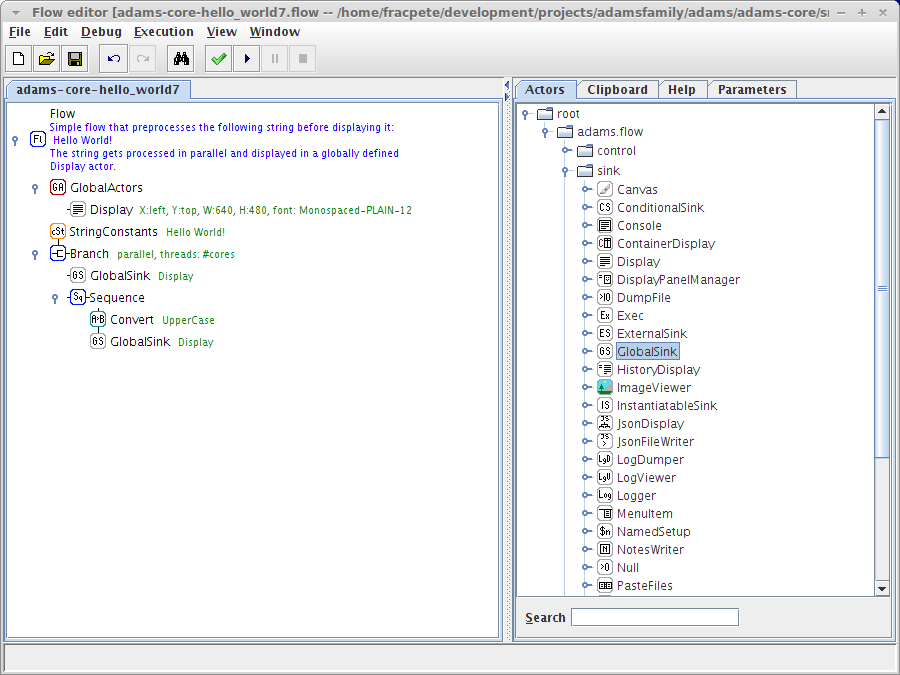
\includegraphics[width=12.0cm]{images/floweditor-helloworld-callable_display.png}
  \caption{Outputting parallel processed strings in a single callable
  \textit{Display} actor.}
  \label{floweditor-helloworld-callable_display}
\end{figure}
In addition to the \textit{CallableSink} actor, there are also the
\textit{CallableSource} actor (for using the same source multiple times in a flow)
and the \textit{CallableTransformer} actor (for instance for using the same
preprocessing multiple times). They are used in the same fashion as the
\textit{CallableSink} actor that we just introduced.

\heading{Combining views}
The \textit{GridView} standalone allows you to define several graphical actors
to be displayed in a grid layout, by adding them below this actor. This can be 
useful, for instance, if two plots have very different scales and plotting them 
in the same graph wouldn't make much sense. Using \textit{GridView}, you can create 
a plot with two rows and one column for displaying the two \textit{SequencePlotter}
actors below each other. The actors below the \textit{GridView} actor get
referenced from within the flow using \textit{CallableSink} actors.

The \textit{TabView} standalone works just like the \textit{GridView} actor,
but instead of displaying the graphical actors in a grid, they get displayed
in a tabbed pane (in the order they are below the \textit{TabView} actor).

\newpage
\section{External actors}
\label{external_actors}
Flows can quickly become large and complex, with lots of preprocessing
happening in multiple locations. Pretty soon you will realize that certain
preprocessing steps are always the same. The same applies to loading data
(e.g., various benchmark data sets) or writing results back to disk.

To avoid unnecessary duplication of functionality, ADAMS allows you to
\textit{externalize} parts of your flow to be externalized, i.e., stored on
disk. Externalizing an existing sub-flow is very easy, you merely have to
right-click on the actor that you want to save to disk and select
\textit{Externalize\ldots} from the popup menu. A new Flow editor window will
pop up with the currently selected sub-flow copied into, ready to be saved to
disk \footnote{Only actors that implement the \textit{InstantiatableActor}
interface can be externalized directly. All others need to be enclosed in the
appropriate \textit{InstantiatableXYZ} wrapper. Using the
\textit{Externalize\ldots} menu item automatically wraps the actor if
required,}. Once you saved the sub-flow to a file, you have to go back into the
original flow and update the file name of the flow in the external \textit{meta}
actor that replaced the sub-flow.

Here are the available meta actors:
\begin{tight_itemize}
	\item \textit{ExternalFlow} -- for executing complete flows.
	\item \textit{ExternalStandalone} -- for using externalized standalones.
	\item \textit{ExternalSource} -- for incorporating an external source.
	\item \textit{ExternalTransformer} -- for applying an external transformer.
	\item \textit{ExternalSink} -- for processing data in an external sink.
\end{tight_itemize}

Once you have an \textit{ExternalXYZ} actor, you can edit this flow directly by 
selecting the \textit{Edit\ldots} menu item as shown in Figure 
\ref{floweditor-externalactors1_editsubflow}.
\begin{figure}[htb]
  \centering
  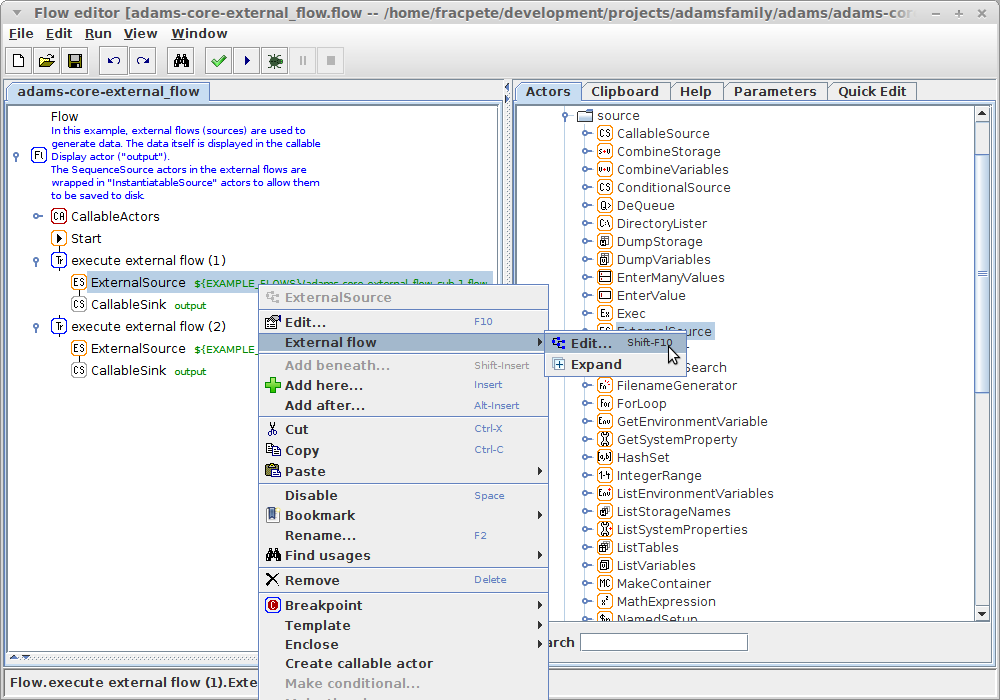
\includegraphics[width=12.0cm]{images/floweditor-externalactors1_editsubflow.png}
  \caption{Editing an external flow directly.}
  \label{floweditor-externalactors1_editsubflow}
\end{figure}

\textbf{Tip:} In the flow editor, you can \textit{inline} an external flow by
selecting \icon{images/expand}\textit{Expand} from the popup menu on the external
actor. This will load the external flow and place it below the external actor
as read-only sub-tree (see Figure \ref{floweditor-externalactors1_expandedsubflow}). You can simply remove the actors using the
\icon{images/collapse}\textit{Collapse} option from the popup menu of the external actor.

\begin{figure}[htb]
  \centering
  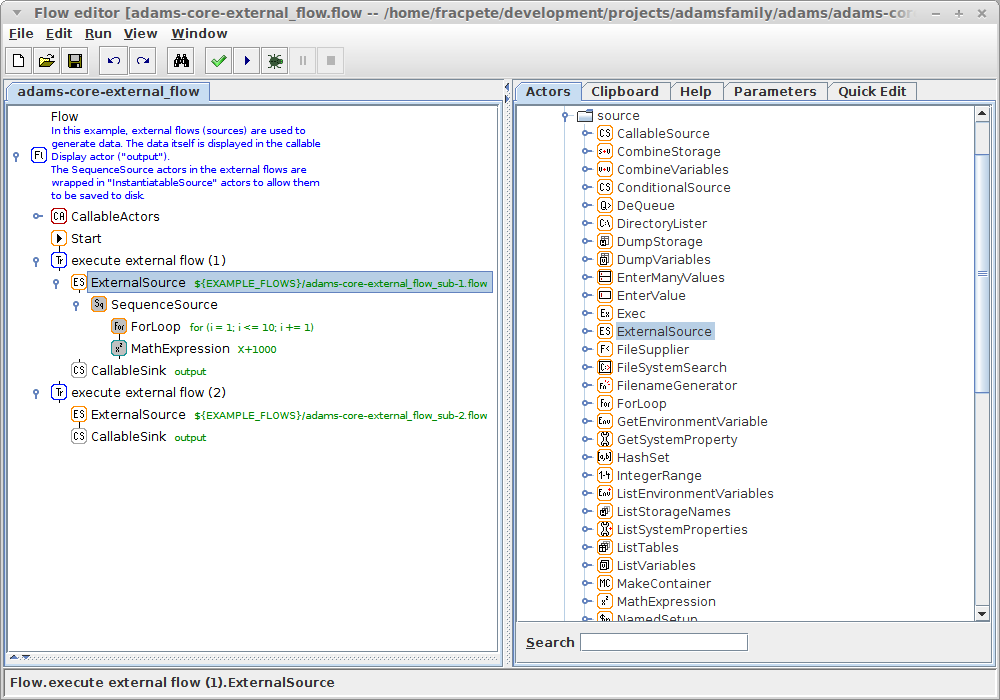
\includegraphics[width=12.0cm]{images/floweditor-externalactors1_expandedsubflow.png}
  \caption{An \textit{inlined} or \textit{expanded} external flow.}
  \label{floweditor-externalactors1_expandedsubflow}
\end{figure}

\newpage
\section{Interactive actors}
\label{interactive_actors}
Most of the times, flows that you generate will simply be executed, without any
user interaction. However, sometimes user interaction can be very useful in
making the flow easier to use. Imagine a flow that takes a file as input, e.g.,
using the \textit{SingleFileSupplier} source, reads and processes it. If the
file varies, you will have to change the source actor each time you want to run
the flow with a different file. To address this shortcoming, ADAMS offers a
range of interactive actors:
\begin{tight_itemize}
	\item \textit{EnterValue} (source) -- allows the user to enter a value or
	choose from a range of options.
	\item \textit{EnterManyValues} (source) -- allows the user to enter one
	or more values, supporting various data types.
	\item \textit{PasteFromClipboard} (source) -- Forwards the content (if any) of
	the system's clipboard (\textit{CopyToClipboard} allows you to copy textual
	data to the system's clipboard).
	\item \textit{SelectArraySubset} (transformer) -- prompts the user to select
	a subset of array elements to be forwarded.
	\item \textit{SelectDateTime} (source) -- pops up a dialog for selecting a
	date/time, date or time, depending on configuration.
	\item \textit{SelectCharset} (source) -- prompts the user to select a
	character set (eg used for file encoding).
	\item \textit{SelectDirectory} (source) -- pops up a dialog for selecting a
	directory.
	\item \textit{SelectFile} (source) -- allows the user to select one or more
	files. File extensions for narrowing down the list of files being displayed is
	possible as well.
	\item \textit{ConfirmationDialog} (transformer) -- prompts the user with a
	dialog, offering ``yes'' and ``no'' as options. If not custom string tokens are
	defined for the ``yes''/''no'' actions, the current token will be forwarded in
	case of the user selecting ``yes'' (``no'' simply drops the token).
	\item \textit{Inspect} (transformer) -- allows the user to view the content
	of a token with the specified panel provider, e.g., image viewer.
\end{tight_itemize}
Using the \textit{SelectFile} source in your flow now, the user won't have to
modify the flow anymore. It is now far less likely that the user accidentally
modifies and breaks the flow in the process.

The source actors allow you to specify \textit{default} values, e.g., a
default directory and default file(s) in case of the \textit{SelectFile} actor.
This cuts down the time the user has to spend clicking through directories in
the file chooser dialog.

Some of these interactive actors can be switched to ``silent'' mode, i.e.,
non-interactive. Counterinuitive as it seems, a rather handy feature when
developing a the flow and constant dialogs are simply too annoying. Once
development of the flow has finished, the non-interactive setting can be
reversed again. You can either set the \textit{nonInteractive} flag for each of
these actors manually, or use the flow editor's menu to either turn the
interactive nature on or off (``Edit'' $\rightarrow$ ``Interactive actors'').

\begin{figure}[htb]
  \centering
  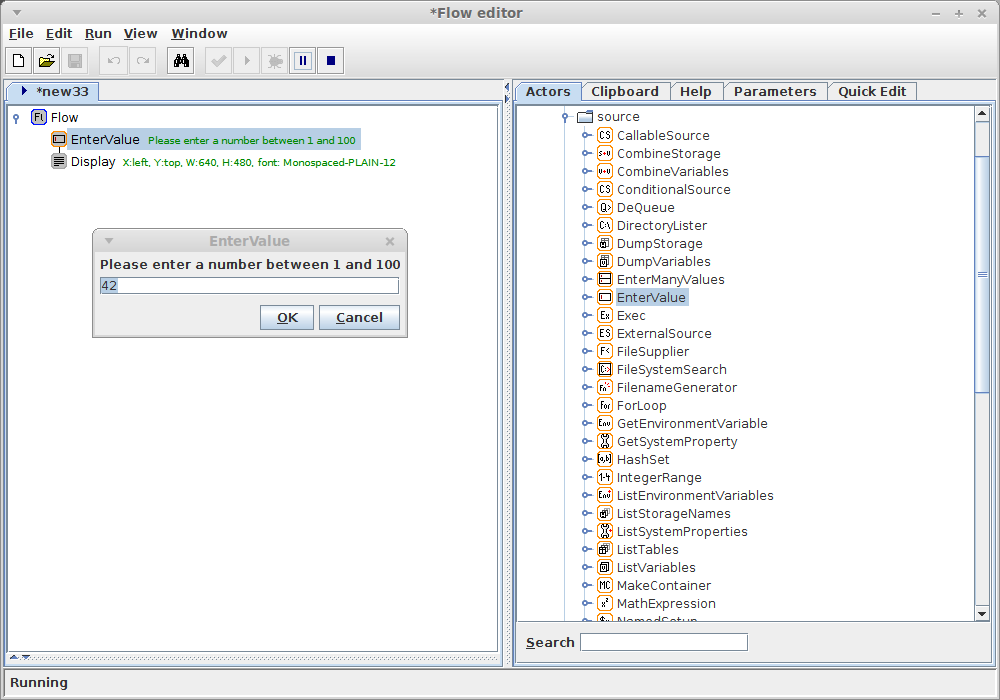
\includegraphics[width=12.0cm]{images/floweditor-interactive_actors1.png}
  \caption{Simple flow that prompts the user to enter a value, using a default
  value of ``42'' and a custom message.}
  \label{floweditor-interactive_actors1}
\end{figure}

\newpage
\section{Templates}
\label{templates}
ADAMS comes with a powerful templating mechanism, that speeds up the
inception of new flows. Templates allow you to insert complete sub-flows
that are generated by a template class. Therefore, commonly occurring sub-flows
can be encapsulated in a template class with optional parameters. A fairly
common sub-flow, encapsulated by a \textit{Trigger} control actor, is the
updating of a variable. The \textit{UpdateVariable} template inserts such a
sub-flow, consisting of a \textit{Variable} source and a \textit{SetVariable}
transformer, enclosed by a \textit{Trigger}. You only need to supply the
variable name that needs updating to generate the sub-flow and then add the
required transformers that take the current variable value and process is some
way or the other. Figures \ref{template-static_use1} to
\ref{template-static_use3} show the use of this mechanism.

\begin{figure}[htb]
  \centering
  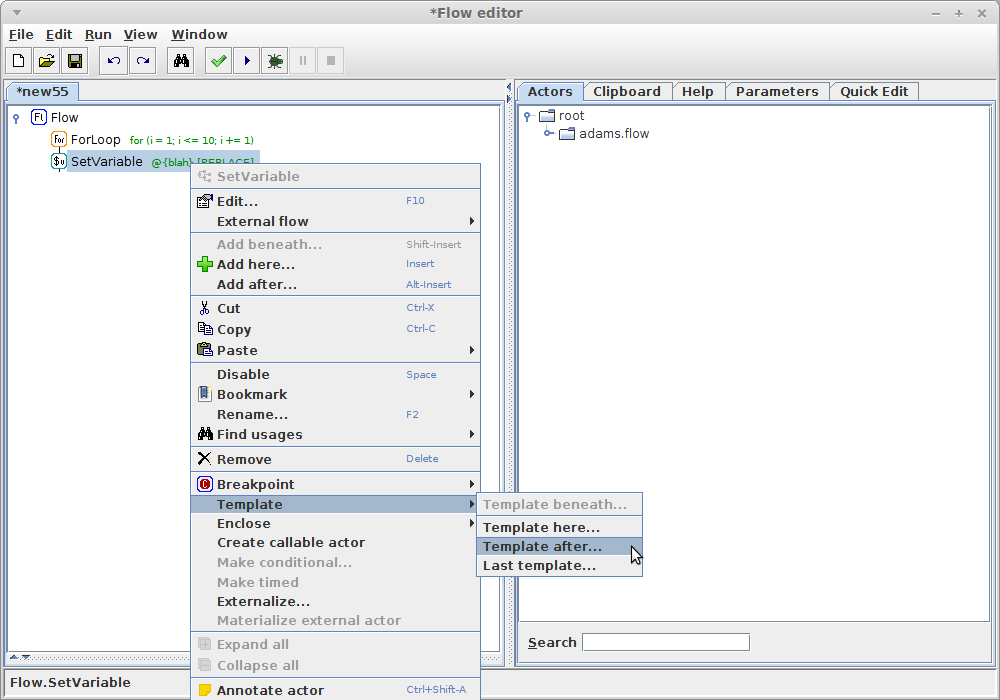
\includegraphics[width=12.0cm]{images/template-static_use1.png}
  \caption{Adding a sub-flow generated from a template to an existing flow.}
  \label{template-static_use1}
\end{figure}

\begin{figure}[htb]
  \centering
  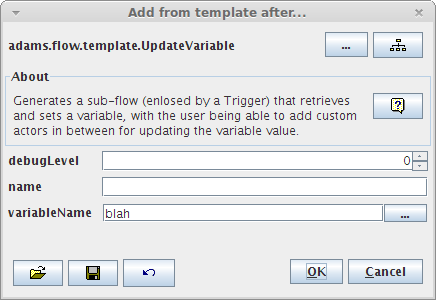
\includegraphics[width=7.0cm]{images/template-static_use2.png}
  \caption{The options of the \textit{UpdateVariable} template.}
  \label{template-static_use2}
\end{figure}

\begin{figure}[htb]
  \centering
  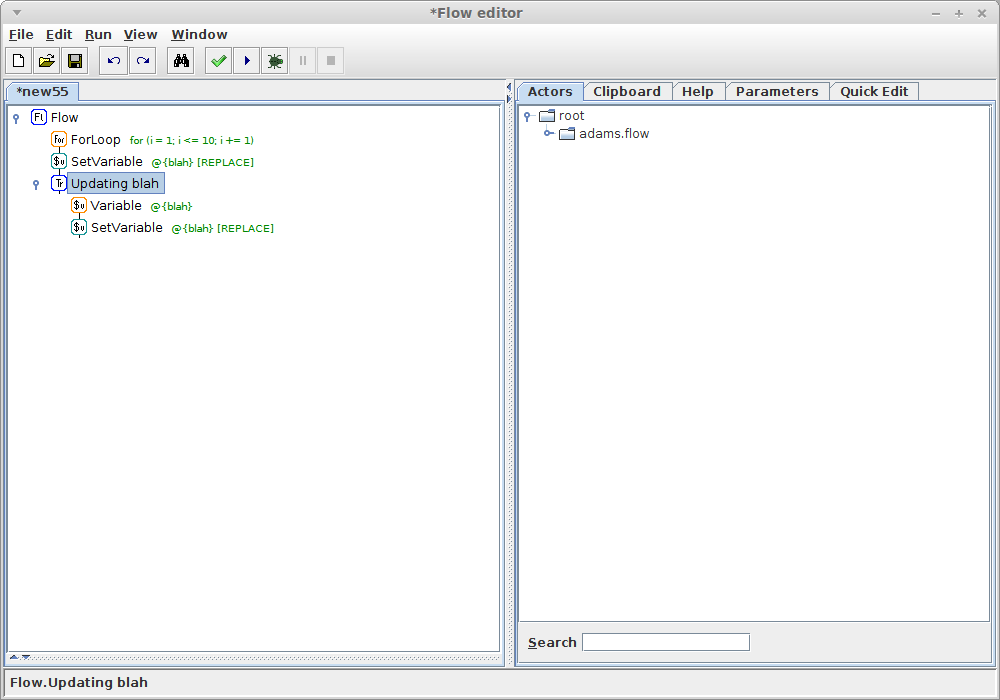
\includegraphics[width=12.0cm]{images/template-static_use3.png}
  \caption{The added sub-flow.}
  \label{template-static_use3}
\end{figure}
The ``adams-meta'' module allows you to use these templates also at runtime,
dynamically generating flows on-the-fly using special actors.

\newpage
\section{Variables}
\label{variables}
A flow is very useful for documenting all the steps involved in loading,
processing and evaluating of data. But setting up a new flow, whenever you are
merely varying a parameter is not very efficient. In order to make flows more
flexible and dynamic, ADAMS offers the concept of \textit{variables}. The
idea of variables is to \textit{attach} them to options of the object that you
want to vary. Actors keep track of what variables have been attached to
themselves or nested objects. Whenever an actor gets executed, it checks first
whether any of the variables that it is monitoring has been modified. If that is
the case, the actor re-initializes itself before the execution takes place. This
guarantees that the correct set up has been applied. At the time of writing,
the scope of variables is restricted to \textit{Flow} actors. Running the same
flow in two concurrent Flow editor windows does not result in those two flows interfering
with each other. In case of attaching variables to options that are arrays,
the variable is expected to be a \textit{blank-separated list} of values.

In the following example \footnote{adams-core-variables1.flow}, we are using a
\textit{ForLoop} source to generate the index of a file to load. In a
\textit{Tee} actor we first convert the integer token to a string using the
\textit{Convert} transformer and the \textit{AnyToString} conversion scheme.
Then we add, first the path and then the file extension, to generate the full
file name using \textit{StringReplace} transformers. Finally, we associate
the generated file name with the variable \textit{filename} using the
\textit{SetVariable} transformer.

In order to display the content of the files, we need to set up a sub-flow that
consists of a \textit{SingleFileSupplier} source, the \textit{TextFileReader}
transformer for reading in the content and a \textit{HistoryDisplay} sink for
displaying the file contents. The sub-flow gets enclosed by a \textit{Trigger}
control actor, which will get executed whenever an integer token from the
\textit{ForLoop} passes through.

To make use of the variable \textit{filename}, we need to attach it to the
\textit{file} option of the \textit{SingleFileSupplier}. You can attach a
variable by simply bringing up the properties editor of an actor (or other
ADAMS object), right-click on the name of the option and then entering the name
of the variable (without ``$@\{$'' and ``$\}$''). The properties editor
indicates whether a variable has been attached to an option by appending an asterisk
(``$*$'') to the name of the option, as can be seen in Figure
\ref{floweditor-variables1_flow-detail}.
\begin{figure}[htb]
  \centering
  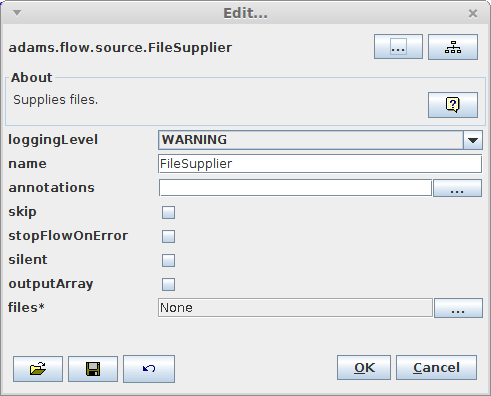
\includegraphics[width=6.0cm]{images/floweditor-variables1_flow-detail.png}
  \caption{The asterisk (``$*$'') next to an option indicates that a variable is
  attached.}
  \label{floweditor-variables1_flow-detail}
\end{figure}

The complete flow is displayed in Figure \ref{floweditor-variables1_flow}. With
``quick info'' enabled, the \textit{SingleFileSupplier} now also hints that the
file it is forwarding is variable-based: \textit{@\{filename\}}.
\begin{figure}[htb]
  \centering
  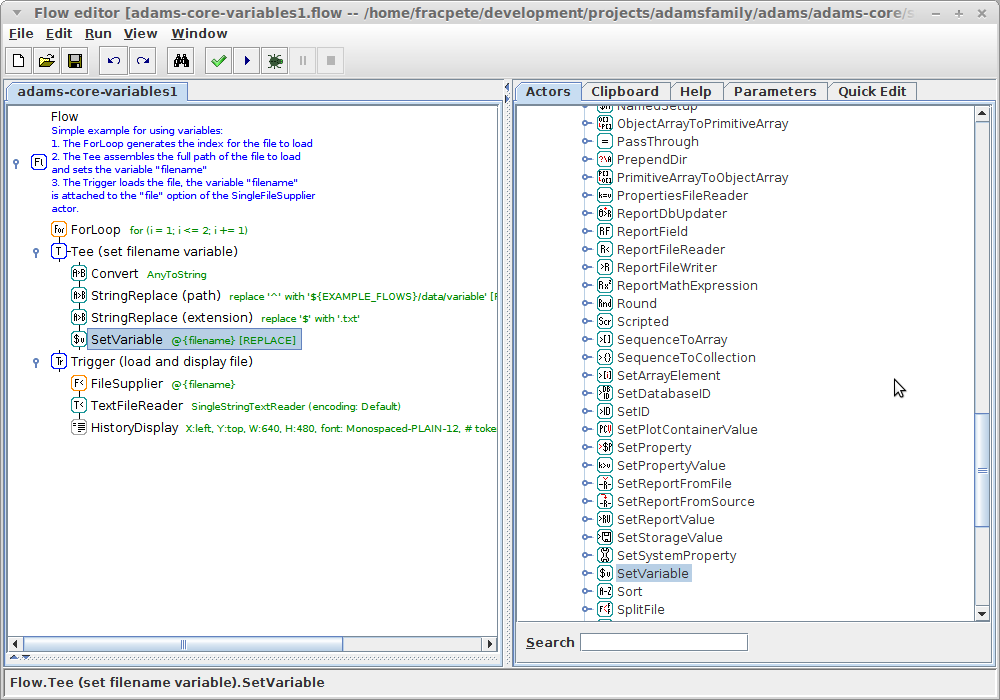
\includegraphics[width=12.0cm]{images/floweditor-variables1_flow.png}
  \caption{Using a variable to control what file to load and display.}
  \label{floweditor-variables1_flow}
\end{figure}

The variable mechanism can also be used to dynamically execute another external
actor at runtime (see section \ref{external_actors} on external actors).

In Figure \ref{floweditor-variables2_flow} you can see a flow that uses a
\textit{ForLoop} to execute three external flows using a variable attached to
the \textit{actorFile} option.
\begin{figure}[htb]
  \centering
  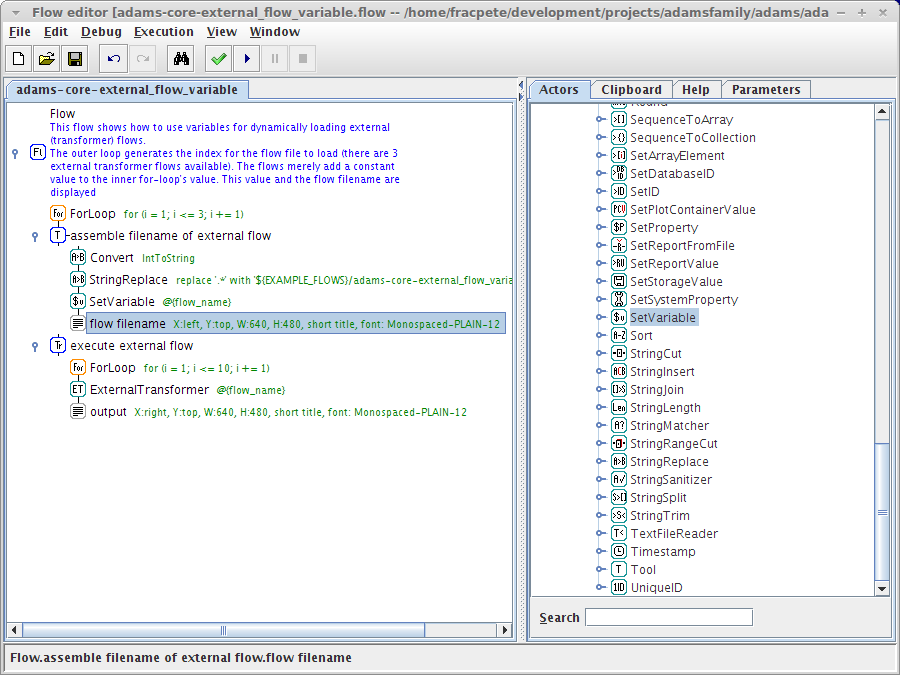
\includegraphics[width=12.0cm]{images/floweditor-variables2_flow.png}
  \caption{Using a variable to control what external flow to execute (flow).}
  \label{floweditor-variables2_flow}
\end{figure}

The output generated by the three sub-flows is shown on screen in the same
\textit{Display} actor. A screenshot of the output is displayed in Figure
\ref{floweditor-variables2_output}.
\begin{figure}[htb]
  \centering
  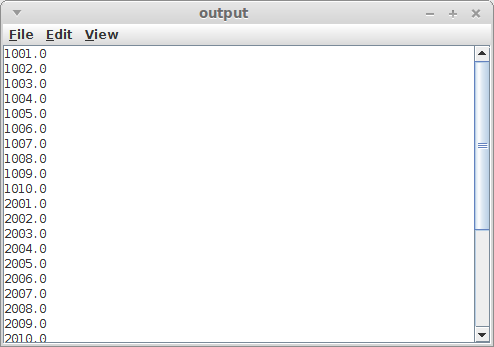
\includegraphics[width=6.0cm]{images/floweditor-variables2_output.png}
  \caption{Using a variable to control what external flow to execute (output).}
  \label{floweditor-variables2_output}
\end{figure}

\heading{Overview of actors}
The following actors are available to handle variables:
\begin{tight_itemize}
	\item \textit{ListVariables} -- source actor for outputting the names of 
	currently available variables.
	\item \textit{DumpVariables} -- source actor for outputting a spreadsheet with
	variable names and their associated values.
	\item \textit{CombineVariables} -- source actor for combining one or more
	variables into a single string using a supplied expression.
	\item \textit{Variable} -- source actor for outputting the value associated
	with the variable.
	\item \textit{VariablesArray} -- outputs the associated values of several
	variables as a string array (source).
	\item \textit{ExpandVariables} -- similar to the \textit{CombineVariables}
	source, this actor expands all variables in the string(s) passing through.
	\item \textit{SetVariable} -- updates the value of a variable (transformer).
	\item \textit{IncVariable} -- increments the value of the variable by either an
	integer or double increment (transformer).
	\item \textit{DeleteVariable} -- removes a variable and its associated value
	from internal memory (transformer).
	\item \textit{ContainerToVariables} -- turns all container values into variables
	that match the specified regular expression (transformer).
	\item \textit{ReportToVariables} -- turns all report values into variables
	that match the specified regular expression (transformer).
\end{tight_itemize}

\heading{Using callable actor as variables}
One drawback of ADAMS is the absence of multiple inputs, only a single input is
supported and containers can mitigate that only to a certain degree. Instead of
only using variables values, ADAMS can also harness data generation on-the-fly,
by attaching callable actors to options. Attaching a callable actor works just like
attaching a simple variable, only the naming convention is different:
\begin{verbatim}
  @{callable:<callable-actor-name>}
\end{verbatim}
The \texttt{callable:} prefix tells ADAMS that the following name is referencing a
callable actor. It then locates the actor and executes it to obtain the value for
using with the option in question.

This mechanism has mainly three caveats:
\begin{tight_itemize}
	\item The callable actor (or sequence of actors) gets executed whenever the
	actor, which has one or more callable actor references attached, gets executed.
	Depending on the actors in use, this can be rather computationally expensive.
	\item Since the variable mechanism has no notion of \textit{where} in the flow
	it is, only callable actors that are defined below the \textit{Flow} actor can be
	used (kind of ``super callable actors'').
	\item The callable actor should generate the correct type for the option it is
	attached to. Otherwise, the value gets converted and parsed as a command-line
	value. Though the flow will be able to recover, this will slow things down
	as an exception will get output whenever this occurs.
\end{tight_itemize}

\heading{Using storage items as variables}
Similar to attaching callable actors, storage values can be attached like
variables as well. Once again, a custom prefix, ``storage'', is used to
distinguish these special variables from ordinary ones:
\begin{verbatim}
  @{storage:<storage-value-name>}
\end{verbatim}
The referenced object is then obtained from storage and set.

This mechanism has two caveats:
\begin{tight_itemize}
	\item The storage value is retrieved whenever the actor, which has one or more
	storage value references attached, gets executed.
	\item The storage value needs to have the correct type for the option it is
	attached to. Otherwise, the value gets converted and parsed as a command-line
	value. Though the flow will be able to recover, this will slow things down
	as an exception will get output whenever this occurs.
\end{tight_itemize}

\heading{Non-ADAMS objects}
The Variable functionality is only available for objects within the ADAMS
framework, as it requires special option handling. 3rd-party libraries do not
benefit from this functionality directly. But thanks to Java Introspection
\footnote{See
\url{http://download.oracle.com/javase/tutorial/javabeans/introspection/}{} for
more information on Java Introspection.} you can use \textit{property paths} to
access nested properties and update their values. A property path is simply the
names of the various properties concatenated and separated by dots (``.''). In
case of arrays, you simply have to append ``[x]'' to the property with ``x''
being the 0-based index of the array element that you want to access.

The following actors handle properties:
\begin{tight_itemize}
	\item \textit{GetProperty} -- transformer that retrieves the current
	value of a property of the token passing through.
	\item \textit{SetProperty} -- transformer that modifies a single property of a
	callable actor using the string representation of the token passing through.
	\item \textit{UpdateProperty} -- transformer that modifies a single property
	of an object passing through using the specified value.
	\item \textit{UpdateProperties} -- allows you to update multiple properties
	(each property is associated with a particular variable) of the actor that
	this actor manages.
\end{tight_itemize}

\heading{Special variables}
Often, flows use resources that are relative to the flow itself. In order to
make this easier, there are two special variables available at runtime:
\begin{tight_itemize}
	\item \textit{flow\_dir} -- stores the path of the flow
	\item \textit{flow\_filename\_long} -- stores path and file name of the flow
	\item \textit{flow\_filename\_short} -- stores only the file name of the flow
\end{tight_itemize}

\newpage
\section{Temporary storage}
\label{temporary_storage}
Variable handling within ADAMS is a very convenient way of changing parameters
on-the-fly, but it comes at a cost. Values for variables are merely stored as
strings internally and each time an options gets updated this string needs to
get parsed and interpreted. Furthermore, each time the whole actor gets
reinitialized if one its own options or an option of its dependent objects gets
updated. It is strongly advised against using the variables functionality if
they are not actually attached to any options, but only used for keeping track
of values like loop variables.

Instead, ADAMS offers an alternative framework for managing values at runtime:
\textit{temporary storage}. In contrast to variables, values are stored
internally as Java objects, referenced by a unique name. Just like with
variables, the scope of these objects is restricted to \textit{Flow} actors at
the time of writing. Additionally, the values don't need to be parsed again
when used, since they are stored as is, resulting in a more efficient
storage/retrieval. Finally, arbitrary objects can be stored, not just objects
for which a string representation can be generated/parsed. The latter aspect
combined with fast storage/retrieval encourages multiple read/write accesses of
the same object in various locations of the flow. An example would be accessing
a data set or spreadsheet, retrieving, setting or updating values. Figure
\ref{floweditor-storage1_flow} shows a flow that takes the number generated by
the random number generator and stores it, before re-using it in the sub-flow
below the \textit{Trigger} actor. The resulting output is displayed in Figure
\ref{floweditor-storage1_output}.

\begin{figure}[htb]
  \centering
  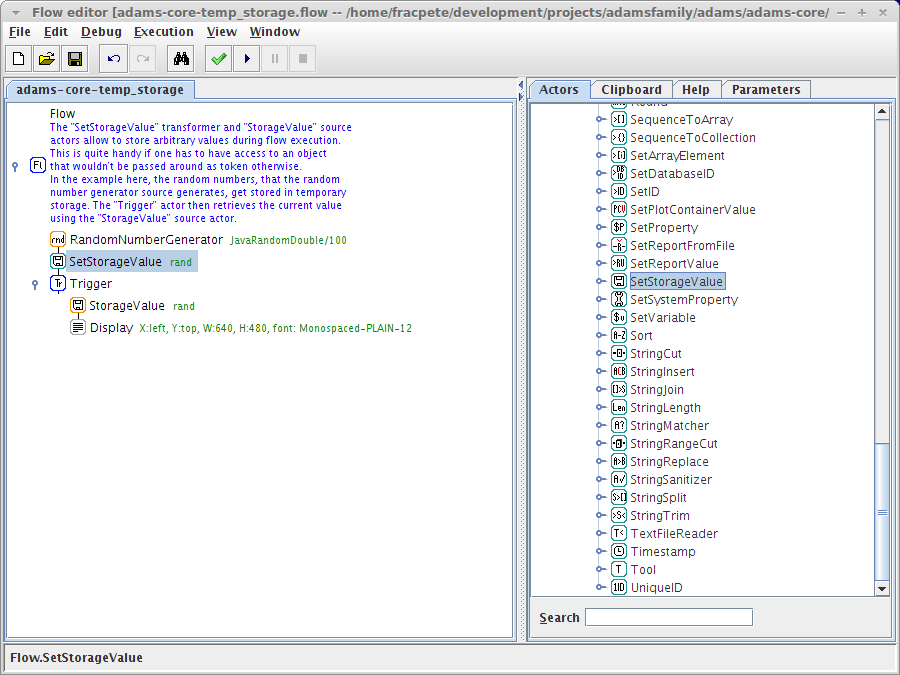
\includegraphics[width=12.0cm]{images/floweditor-storage1_flow.png}
  \caption{Flow demonstrating the temporary storage functionality.}
  \label{floweditor-storage1_flow}
\end{figure}

\begin{figure}[htb]
  \centering
  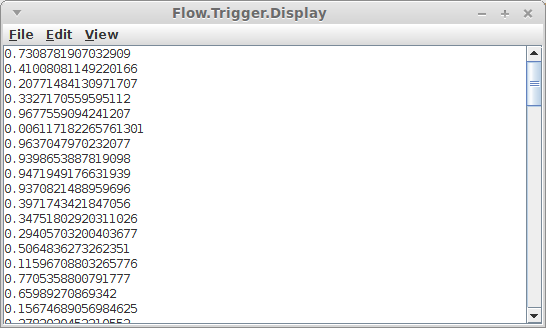
\includegraphics[width=6.0cm]{images/floweditor-storage1_output.png}
  \caption{Output of flow demonstrating the temporary storage
  functionality.}
  \label{floweditor-storage1_output}
\end{figure}

By default, the storage system is unlimited which can quickly result in memory
problems when not used wisely. In order to restrict memory usage and encourage
re-generation of values on demand, the storage system also offers
least-recently-used (LRU) caches \footnote{See
\url{http://en.wikipedia.org/wiki/Cache_algorithms\#Least_Recently_Used}{} for
more information on LRU caches.}. Instead of simply setting a value with a name,
you can specify the name of a particular LRU cache as well. The cache needs to
be initialized first, of course, using the \textit{InitStorageCache} standalone
actor. Figure \ref{floweditor-storage2_flow} shows the use of the LRU cache
functionality, with Figure \ref{floweditor-storage2_inspectionpanel} displaying
a snapshot in time of the storage inspection panel available through the
\textit{Breakpoint} control actor. Finally, Figure
\ref{floweditor-storage2_output} shows the final output of the flow.

\begin{figure}[htb]
  \centering
  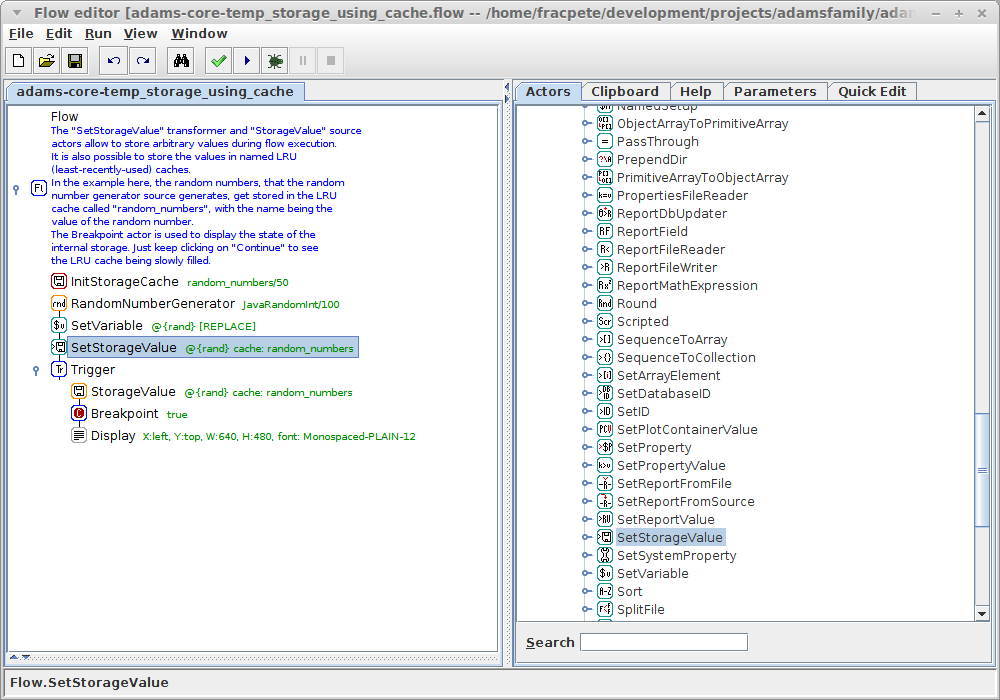
\includegraphics[width=12.0cm]{images/floweditor-storage2_flow.png}
  \caption{Flow demonstrating the LRU cache storage functionality.}
  \label{floweditor-storage2_flow}
\end{figure}

\begin{figure}[htb]
  \centering
  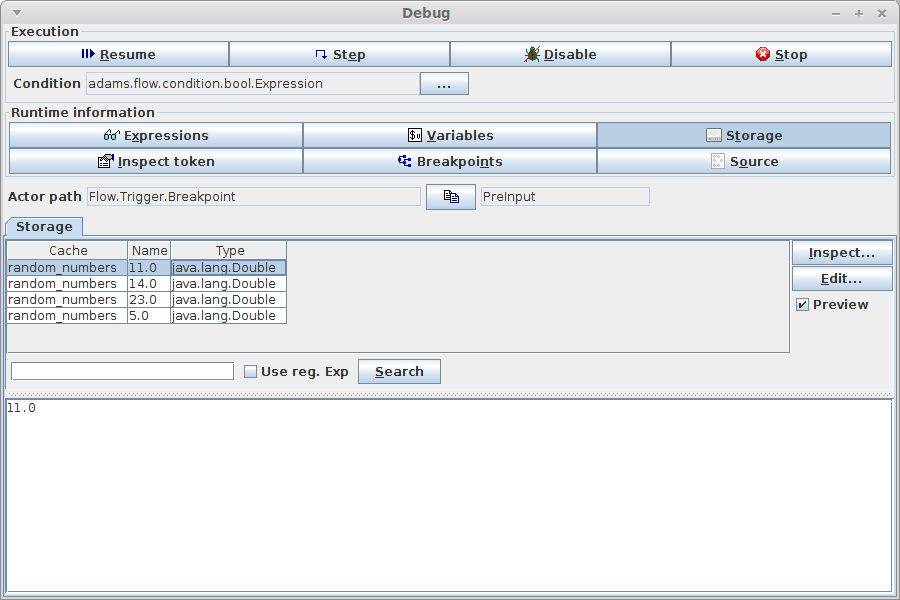
\includegraphics[width=12.0cm]{images/floweditor-storage2_inspectionpanel.png}
  \caption{Display of the temporary storage during execution.}
  \label{floweditor-storage2_inspectionpanel}
\end{figure}

\begin{figure}[htb]
  \centering
  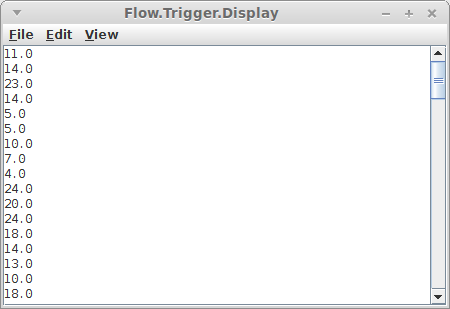
\includegraphics[width=5.0cm]{images/floweditor-storage2_output.png}
  \caption{Output of flow demonstrating the LRU cache storage
  functionality.}
  \label{floweditor-storage2_output}
\end{figure}

\heading{Overview of actors}
The following actors are available to handle variables:
\begin{tight_itemize}
	\item \textit{InitStorageCache} -- standalone actor for initializing a named
	LRU cache with a specific size.
	\item \textit{CombineStorage} -- source actor for combining string 
	representations of storage items and variables into a string.
	\item \textit{ExpandStorage} -- similar to the \textit{CombineStorage}
	source, this actor expands all storage items and variables in the string(s) 
	passing through.
	\item \textit{GetStorageValue} -- transformer that replaces the incoming 
	string with the storage value that the string represents.
	associated with the specified name.
	\item \textit{ListStorageNames} -- source actor for outputting the names of 
	the currently stored items.
	\item \textit{DumpStorage} -- source actor for outputting the names of
	the currently stored items and their associated values (in string
	representation) in a spreadsheet.
	\item \textit{StorageValue} -- source actor for outputting the storage value
	associated with the specified name.
	\item \textit{StorageValuesArray} -- source actor for outputting the 
	storage values associated with the specified names as an array.
	\item \textit{SetStorageValue} -- updates the specified storage value
	(transformer).
	\item \textit{IncStorageValue} -- increments the value of the stored integer or
	double object by either an integer or double increment (transformer).
	\item \textit{DeleteStorageValue} -- removes a storage value
	from internal memory (transformer), freeing up memory.
	\item \textit{ContainerToStorage} -- places all the container values in storage
	that match the regular expression (transformer).
	\item \textit{ReportToStorage} -- places all the report values in storage
	that match the regular expression (transformer).
\end{tight_itemize}


\newpage
\section{Debugging your flow}
\label{debugging_flow}
\subsection{Breakpoints}
The more complex a flow gets, the harder it becomes to track down problems. With
all its general purpose actors and control actors (loops, switch, if-then-else,
\ldots), ADAMS is basically a basic graphical programming language. A
programming language without at least some basic debugging support is very
inconvenient. Therefore, ADAMS allows you to set \textit{breakpoints} in your
flow. These breakpoints are merely instances of the \textit{Breakpoint} control
actor. This actor allows you to specify a breakpoint condition on when to stop.
The default condition is \textit{true}, i.e., the execution gets paused whenever
the actor gets reached. This boolean condition can also evaluate the value of
variables. Just surround the name of the variable with ``@\{'' and ``\}'' in
order to use its value within the expression. For more information on what the
expression can comprise of, check the online help of the \textit{Breakpoint}
actor.

Whenever a \textit{Breakpoint} actor is reached and the condition evaluates to
\textit{true}, the debugging control panel will get displayed (see Figure
\ref{floweditor-debugging1_controlpanel}).
\begin{figure}[htb]
  \centering
  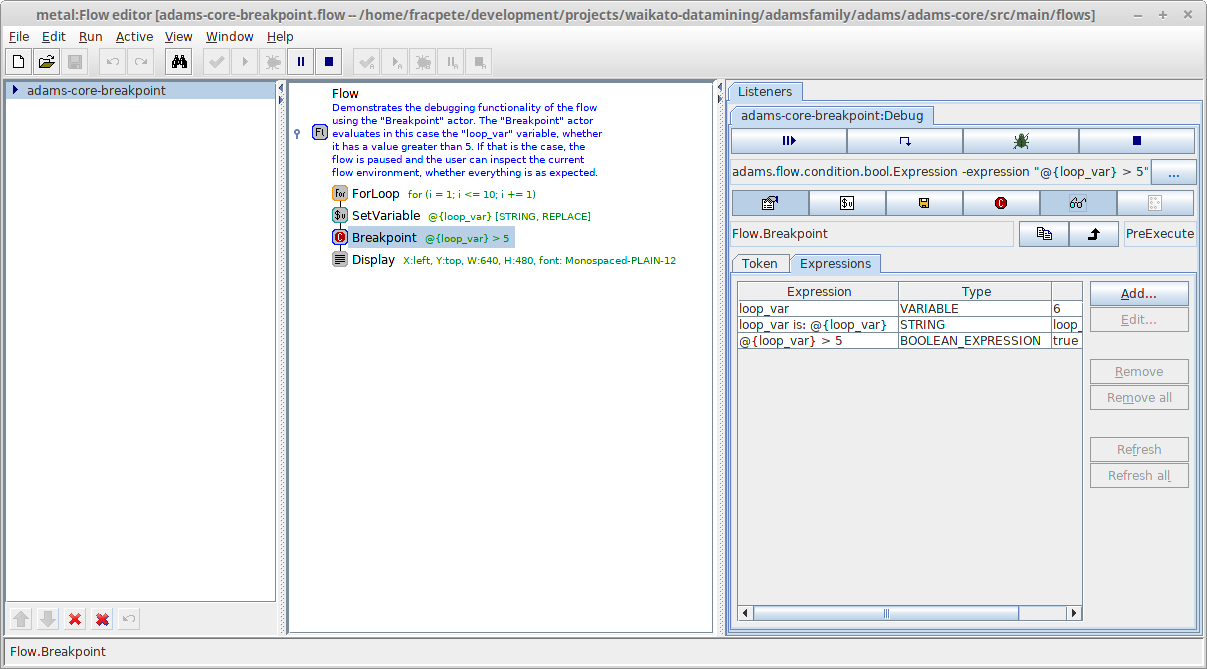
\includegraphics[width=12.0cm]{images/floweditor-debugging1_controlpanel.png}
  \caption{The debugging control panel.}
  \label{floweditor-debugging1_controlpanel}
\end{figure}

The functionality of the control panel is best explained with an example. The
flow \footnote{adams-core-breakpoint.flow} in
Figure \ref{floweditor-debugging1_flow} simply outputs integer values, ranging
from 1 to 10. This value gets stored in the variable \textit{loop\_var} which is
also part of the condition of the \textit{Breakpoint} actor. Finally, these
values get displayed in a \textit{Display} sink.
\begin{figure}[htb] 
  \centering
  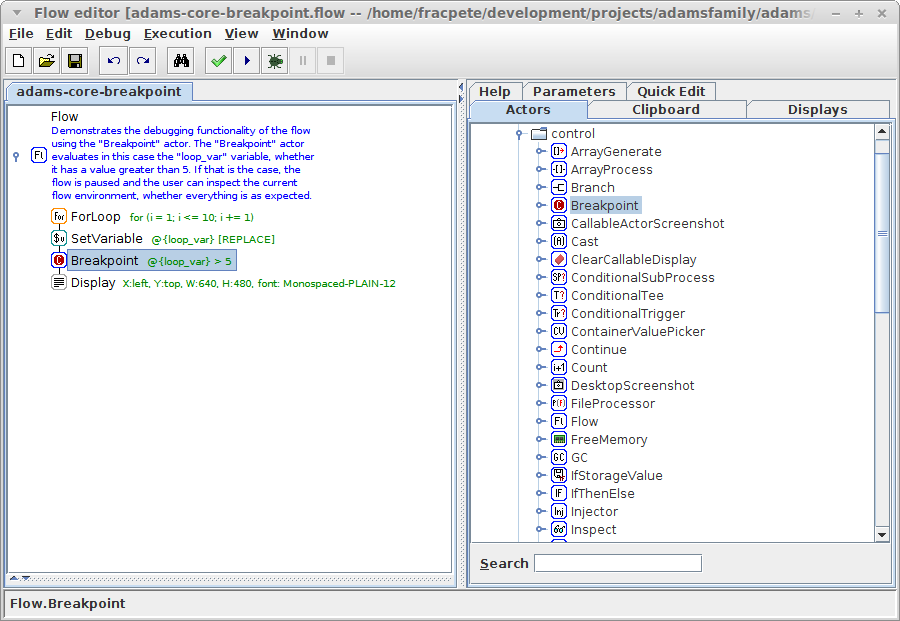
\includegraphics[width=12.0cm]{images/floweditor-debugging1_flow.png}
  \caption{Example flow with \textit{Breakpoint} actor.}
  \label{floweditor-debugging1_flow}
\end{figure}

When the breakpoint gets triggered, the flow gets paused and the aforementioned
control panel is displayed.
\begin{tight_itemize}
	\item The buttons in the \textit{Execution} group allow you to
	resume the flow execution, step through it, actor by actor,
	stop the flow or simply disable the current breakpoint.
	\item It is possible to update the breakpoint condition whenever the breakpoint
	is reached.
	\item In the \textit{Runtime information} group you can view the source code of
	the fully expanded flow (i.e., all external actors are inserted completely and
	variables are expanded to their current value), you can define watch
	expressions (variables, boolean and numeric expressions; Figure
	\ref{floweditor-debugging1_controlpanel}), display an overview of all the
	variables and their current values, inspect the current storage
	items, you can inspect the current token that is being passed through the
	breakpoint (Figure \ref{floweditor-debugging1_inspectionpanel}) and also
	all breakpoints currently present in the flow (Figure
	\ref{floweditor-debugging1_breakpoints}). Breakpoints can be disabled
	and enabled, modified when to stop.
\end{tight_itemize}

\begin{figure}[htb]
  \centering
  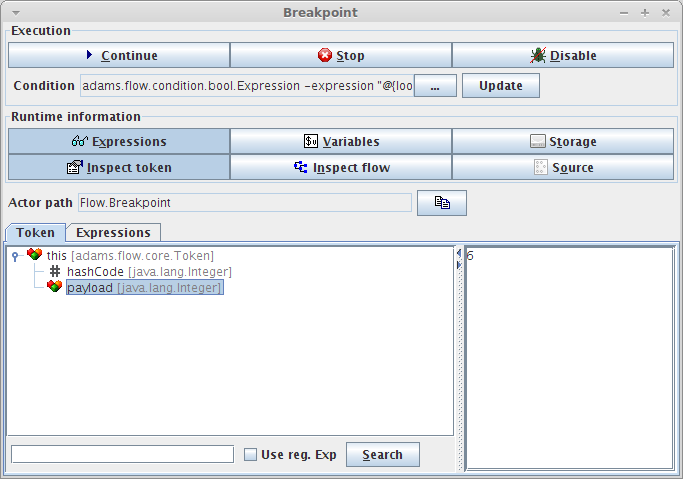
\includegraphics[width=12.0cm]{images/floweditor-debugging1_inspectionpanel.png}
  \caption{The \textit{Inspection} tab of the debugging control panel for the current token.}
  \label{floweditor-debugging1_inspectionpanel}
\end{figure}

\begin{figure}[htb]
  \centering
  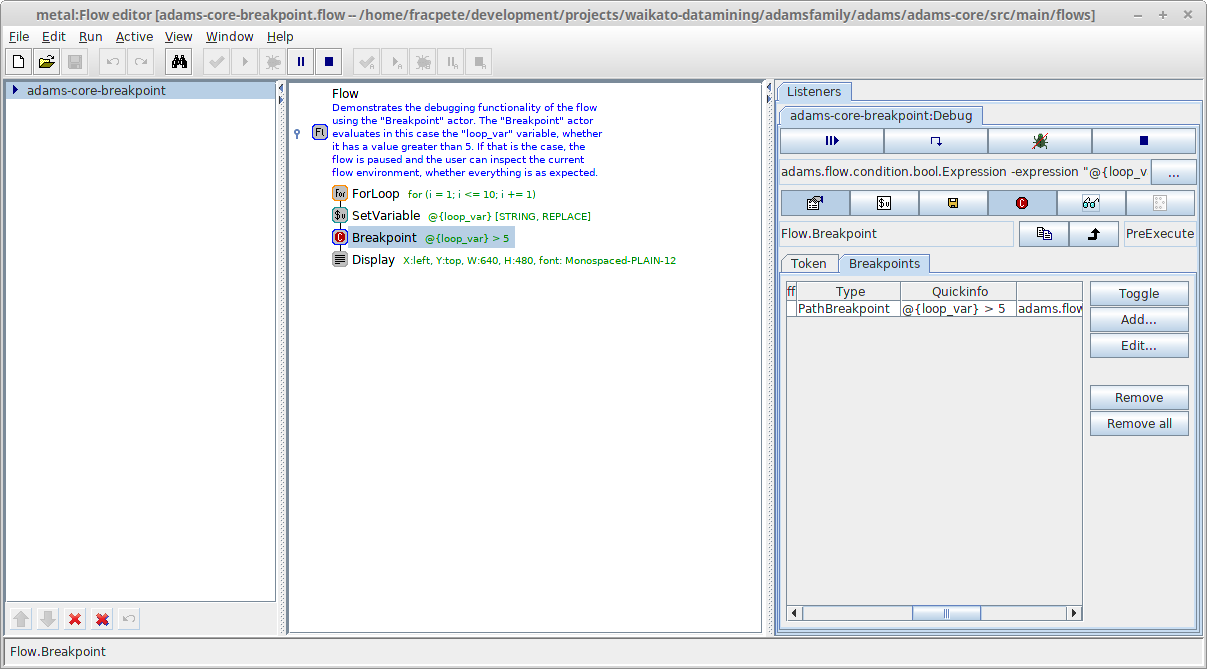
\includegraphics[width=12.0cm]{images/floweditor-debugging1_breakpoints.png}
  \caption{The \textit{Breakpoints} tab of the debugging control panel.}
  \label{floweditor-debugging1_breakpoints}
\end{figure}

While a flow is running, you have some basic tools for inspection at hand as 
well (available from the \textit{Run} menu):
\begin{tight_itemize}
	\item \textit{Variables} -- allows you to monitor the variables of a flow
	and how they change. Note that updating the dialog is quite expensive and
	will slow down your flow considerably.
	\item \textit{Storage} -- when a flow is paused, you can inspect the 
	current storage items; as soon as you resume the flow, the dialog will 
	disappear again, as it doesn't get refreshed automatically.
\end{tight_itemize}
A breakpoint can be triggered at various stages of executing an actor:
\begin{tight_itemize}
  \item pre/post input of a token (transformers, sinks)
  \item pre/post execute
  \item pre/post output of a token (sources, transformers)
\end{tight_itemize}
Inspecting a token is only available at stages \textit{preInput},
\textit{postOutput} and possibly at \textit{preExecute}, if the
actor is a transformer or sink.

Stepping through a flow, using the \textit{Step} button from the control
panel, always uses the \textit{preExecute} stage (\textit{pre/postInput}
are not available, unfortunately due to API limitations).

\subsection{Monitoring}
With ADAMS it is possible to \textit{eavesdrop} on the flow execution by 
attaching a so-called \textit{flow execution listener} to the \textit{Flow}
actor and enable the listening process there as well.

The following listeners are available:
\begin{tight_itemize}
	\item \textit{CurrentlyExecuted} -- displays all the actors (with their 
	start times) that are currently being executed.
	\item \textit{Debug} -- the \textit{Breakpoint} control actors use
	this listener, setting the appropriately configured breakpoints.
	\item \textit{ExecutionCounter} -- counts for each actor how often it was
	executed.
	\item \textit{ExecutionLog} -- writes all calls to the input, execute 
	and output methods to a log file.
	\item \textit{MultiListener} -- allows you to listen with multiple 
	listener setups to the flow execution.
	\item \textit{NullListener} -- dummy listener, does nothing.
\end{tight_itemize}


\newpage
\section{Passwords}
In various places, ADAMS requires the use of passwords, for instance, when
connecting to databases. ADAMS does not offer any proper encryption of the 
passwords, merely a weak obfuscation using 
Base64\footnote{\url{http://en.wikipedia.org/wiki/Base64}{}} encoding. Keep 
this in mind when designing flows and making the available to other people.


\newpage
\section{External processes and classes}
ADAMS allows you to start up external processes or call Java classes that
are present in the classpath from within a flow. The following actors are 
available:
\begin{tight_itemize}
	\item \textit{Java} -- standalone that calls the \textit{main} method of a 
	Java class, using the current JVM.
	\item \textit{JavaExec} -- standalone that starts up a new JVM using
	the current classpath and JRE. stdout and stderr can be further processed
	in the flow.
	\item \textit{Exec} -- source that calls any external executable and allows
	to further process either stdout or stderr.
\end{tight_itemize}

%%%%%%%%%%%%%%%%%
% Visualization %
%%%%%%%%%%%%%%%%%

\chapter{Visualization}
Visualization is very important in data analysis. The core module of ADAMS
comes with some basic support.
\begin{tight_itemize}
	\item \textbf{Image viewer} -- For displaying images of type PNG, JPEG, BMP,
	GIF.
	\item \textbf{Preview browser} -- Generic preview browser, any ADAMS module can
	register new preview handlers for various file types.
\end{tight_itemize}

\section{Image viewer}
The Image viewer is a basic viewer for graphic files (PNG, JPEG, BMP, GIF).
Figure \ref{imageviewer1} shows the viewer with a single image loaded. It is
possible to copy images to the system's clipboard, export or save them in a
different file format or print them.

\begin{figure}[htb]
  \centering
  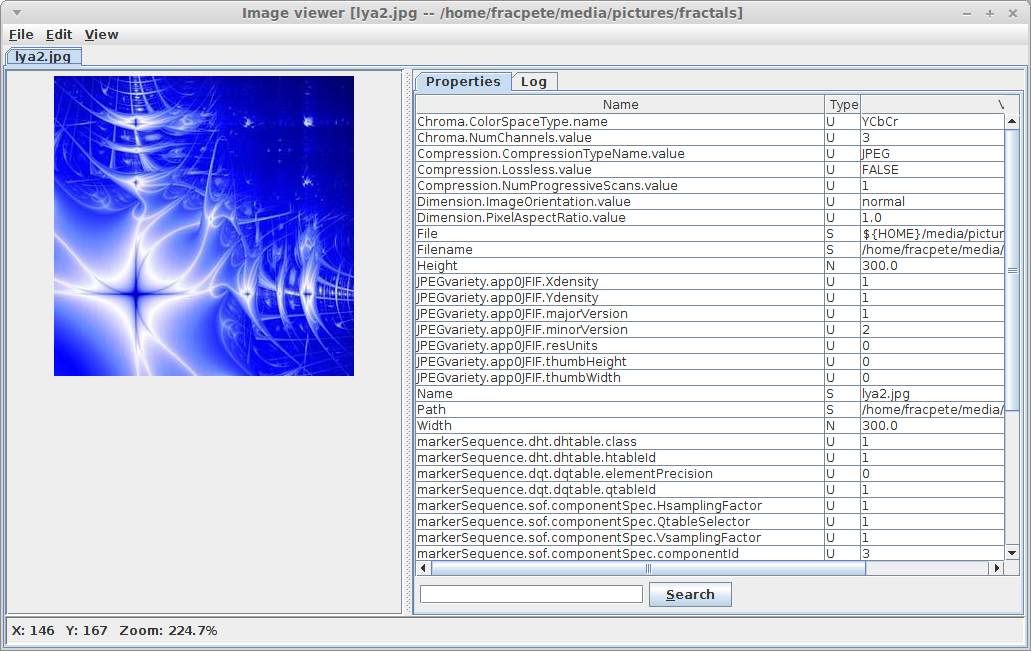
\includegraphics[width=12.0cm]{images/imageviewer1.png}
  \caption{Displaying a fractal in the Image viewer.}
  \label{imageviewer1}
\end{figure}

\section{Preview browser}
The preview browser is a generic preview framework within in ADAMS and each
module can register new handlers for various file or archive types. In its basic
functionality, the preview browser can view images (see
\ref{previewbrowser-image1}), properties files, flows (see
\ref{previewbrowser-flow1}) and plain text files (see
\ref{previewbrowser-plaintext1}). If no handler is registered for a file type,
i.e., a certain file extension, then the plain text handler is used by default.
If more than one handler is registered for a file type, then you can select
from the combobox at the bottom of the dialog, which handler is the preferred
for this type of file.

\begin{figure}[htb]
  \centering
  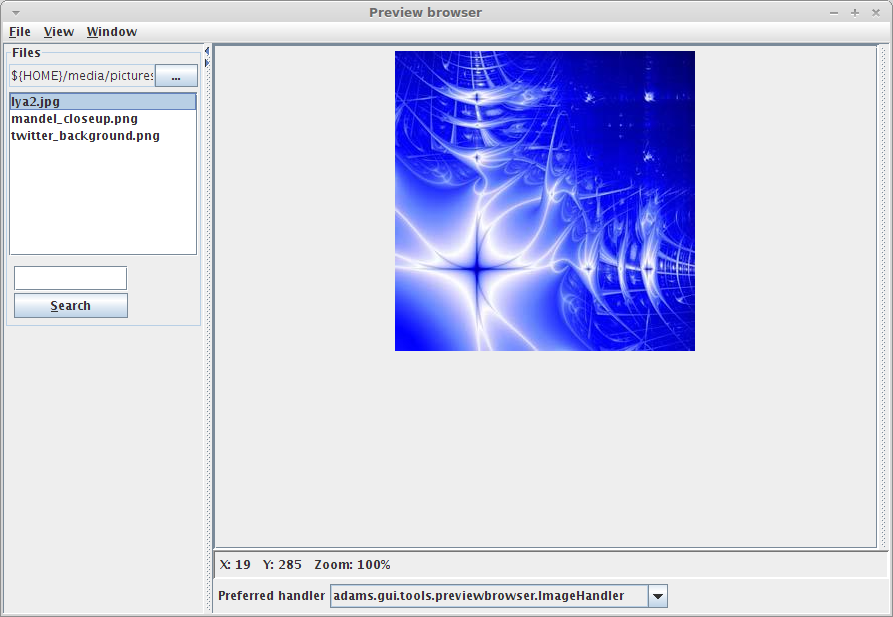
\includegraphics[width=12.0cm]{images/previewbrowser-image1.png}
  \caption{Preview browser displaying an image.}
  \label{previewbrowser-image1}
\end{figure}

\begin{figure}[htb]
  \centering
  \includegraphics[width=12.0cm]{images/previewbrowser-flow1.png}
  \caption{Preview browser displaying a flow.}
  \label{previewbrowser-flow1}
\end{figure}

\begin{figure}[htb]
  \centering
  \includegraphics[width=12.0cm]{images/previewbrowser-plaintext1.png}
  \caption{Preview browser displaying an plain text file.}
  \label{previewbrowser-plaintext1}
\end{figure}

Serialized files can be inspected as well, e.g., for model files generated 
by WEKA. Other modules may offer specific viewers for the objects stored
in such a file.

%%%%%%%%%%%%%%%%%%%
% Remote commands %
%%%%%%%%%%%%%%%%%%%

\chapter{Remote commands}

ADAMS offers a generic framework for remote commands, either uni-directional
ones (e.g., restarting the remote instance) or bi-directional ones
(e.g., retrieving system info from the remote instance).

Uni-directional commands, see Figure \ref{remote_command-uni_directional},
only require the remote instance to \textit{listen} for incoming commands
using a remote scripting engine. Bi-directional ones, on the other hand,
require the local and the remote instance to listen for incoming commands.
Figure \ref{remote_command-bi_directional} shows how the local instance
sends a request to the remote one and then listens for the response to
come in.

\begin{figure}[htb]
  \centering
  \includegraphics[width=8.0cm]{images/remote_command-uni_directional.png}
  \caption{Uni-directional command.}
  \label{remote_command-uni_directional}
\end{figure}

\begin{figure}[htb]
  \centering
  \includegraphics[width=8.0cm]{images/remote_command-bi_directional.png}
  \caption{Bi-directional command (\textit{with response}).}
  \label{remote_command-bi_directional}
\end{figure}

In order to control the remote scripting engine, you can start/stop them
from the main menu: \textit{Program $\rightarrow$ Remote commands...}
The following scripting engines are available:
\begin{tight_itemize}
  \item \textit{DefaultScriptingEngine} -- just listens on a specified
  port for commands.
  \item \textit{FileBasedScriptingEngine} -- polls a directory for incoming
  commands.
  \item \textit{ForwardingScriptingEngine} -- forwards incoming commands
  to a specified connection. Can act as load-balancer or single point of access
  in conjunction with the \textit{LoadBalancer} connection and multiple defined
  sub-connections.
  \item \textit{ManualFeedScriptingEngine} -- only to be used internally, where
  the commands are being added programmatically.
\end{tight_itemize}

From this menu, you can also launch commands using the \textit{Send...}
menu item. The dialog that you get prompted with allows you to configure
the remote command and the type of connection to use to reach the remote
host.

The remote command functionality is not only available from the main menu,
you can also use this functionality within flows, allowing for automation
of tasks. However, you still need to start the remote scripting engine. Though
this can be automated via a command-line option when starting up ADAMS
(\texttt{-remote-scripting-engine-cmdline}) on the remote machine.

Available actors:
\begin{tight_itemize}
  \item \textit{ExecuteRemoteCommand} -- executes the command coming through.
  \item \textit{GetRemoteCommandPayload} -- retrieves the payload objects (if
  any) from a remote command
  \item \textit{NewRemoteCommand} -- configures and forwards a command object.
  \item \textit{RemoteCommandRaeader} -- transformer that reads a command
  object from the incoming file.
  \item \textit{SendRemoteCommand} -- sends the command object across the wire
  using the specified connection setup.
  \item \textit{RemoteCommandWriter} -- writes the incoming command object to disk.
  \item \textit{RemoteScriptingEngine} -- standalone for running a scripting
  engine within the flow.
  \item \textit{TriggerRemoteExecution} -- uses the RemoteFlowExecution command
  to send the sub-flow for remote execution.
\end{tight_itemize}

Available conversions:
\begin{tight_itemize}
  \item \textit{StringToRemoteCommand} -- parses the string and turns it into
  a \textit{RemoteCommand} object
  \item \textit{RemoteCommandToString} -- generates a string representation of
  the remote command (which is used for transmitting across the network)
\end{tight_itemize}

\section{Registering flows}
In order to use the \textit{GetFlow} or \textit{ListFlows} remote commands,
the flows running on the remote server need to be registered with the
registry for \textit{running flows}. This can be achieved in two ways:
\begin{tight_itemize}
  \item \textbf{per flow} -- by using the \textit{RegisterFlow} standalone
  actor in a flow.
  \item \textbf{system-wide} -- by setting the \textit{AutoRegister} property
  in the \textit{adams/flow/control/Flow.props} file to \textit{true}.
\end{tight_itemize}

\section{Linux servers}
ADAMS can be run in a headless environment, i.e., without graphical user
interface. Installing workflows that process data on a Linux server, e.g.,
Ubuntu, is fairly easy:
\begin{tight_itemize}
  \item Create non-privileged user \texttt{adams} and add other users like
  yourself to that user's group in \texttt{/etc/group}.
  \item Add your public RSA key\footnote{Best practice is to create a new
  RSA key pair for this server/application, in case the server gets compromised
  and you need to regenerate the key. The implications of replacing such a
  key-pair are then fairly limited.} to \texttt{/home/adams/.ssh/authorized\_keys}.
  \item Download, extract and copy an Oracle JDK to \texttt{/opt/jdk}
  \item Download, extract and copy ADAMS to \texttt{/opt/adams}
  \item If your flow is processing files, create the directory structure
  (see Figure \ref{example_dir_layout_data_processing} for an example).
  \item Make sure that all files and directories are owned by the \texttt{adams}
  user (using \texttt{chown}) and that the permissions for the \texttt{adams}
  group are set correctly as well (using \texttt{chmod}).
  \item Create the script that will execute your flow, e.g.,
  \texttt{/usr/local/bin/myflow.sh} which executes the flow called
  \texttt{myflow.flow}:
    {\scriptsize
    \begin{verbatim}
unset DISPLAY
cd /opt/adams
/opt/jdk/bin/java -cp "./lib/*" adams.flow.FlowRunner -headless -input ./flows/myflow.flow &
    \end{verbatim}}
  \item Assume the identity of the \texttt{adams} user, e.g., by using
  \texttt{sudo su - adams} and add the following cronjob, using \texttt{crontab -e},
  which will execute your flow at startup time:
    \begin{verbatim}
    @reboot /usr/local/bin/myflow.sh
    \end{verbatim}
\end{tight_itemize}

\begin{figure}[htb]
\dirtree{%
 .1 /.
 .2 opt.
 .3 data.
 .4 incoming \DTcomment{\textrm{for receiving data}}.
 .4 processing \DTcomment{\textrm{currently being processed}}.
 .4 processed \DTcomment{\textrm{successfully processed}}.
 .4 failed \DTcomment{\textrm{failed to process for some reason}}.
}
  \caption{Example directory layout for data processing.}
  \label{example_dir_layout_data_processing}
\end{figure}


%%%%%%%%%
% Tools %
%%%%%%%%%

\chapter{Tools}
Among the items in the \textit{Tools} menu are the most important tools of 
ADAMS, the interfaces for editing and running flows.

\section{File commander}
The \textit{File commander} is a file manager wtih two panes for easy copying,
moving, deleting and viewing of files. It was inspired by the
\textit{Midnight Commander}\footnote{\url{http://www.midnight-commander.org/}{}}.
Figure \ref{filecommander} shows a screenshot.

\begin{figure}[htb]
  \centering
  \includegraphics[width=12.0cm]{images/filecommander.png}
  \caption{File manager interface.}
  \label{filecommander}
\end{figure}

\section{Flow editor}
The Flow editor is the central tool in ADAMS, allowing you the definition of
powerful workflows for a multitude of purposes. See chapter \ref{flows} for a
comprehensive introduction.

\section{Flow runner}
The \textit{Flow runner} is an interface to execute flows without the user
being able to modify them. See chapter \ref{running_flows} for more information.

\section{Actor usage}
The class \textit{adams.flow.core.ActorUsage} allows you to generate a spreadsheet 
that generates an overview of which actors are used in what flows. Here is an example 
command-line for Linux:
\begin{verbatim}
  adams.flow.core.ActorUsage \
    -dir ./flows \
    -recursive \
    -no-path \
    -output $HOME/actors.csv \
    -logging-level INFO
\end{verbatim}
The command looks recursively for flows, starting in the \textit{./flows}
directory. The generated output, omitting the path from the flow files, is 
written to \textit{actors.csv} in the user's home directory.

Rather than using a static spreadsheet, you can also use this tool from the 
main menu: \textit{Help -> Actor usage}. After selecting a directory containing
flows (which will get searched recursively), you will be presented with a dialog
that displays the generated spreadsheet (see Figure \ref{actor_usage}). This
dialog also allows you to select one or more flow files and then edit them,
by clicking on the \textit{Edit} button. You can directly edit a single flow
by double-clicking on it in the table as well.

\begin{figure}[htb]
  \centering
  \includegraphics[width=12.0cm]{images/actor_usage.png}
  \caption{Overview of actor usage in flow files.}
  \label{actor_usage}
\end{figure}

\section{Text editor}
The \textit{Text editor} is a very simply editor for plain text files. It 
allows you to view and edit one file at a time. It also supports printing
and, if the \textit{net} module is present, sending the files via Email.

\begin{figure}[htb]
  \centering
  \includegraphics[width=12.0cm]{images/texteditor.png}
  \caption{Editor for viewing/editing plain text files.}
  \label{texteditor}
\end{figure}

\clearpage
\newpage
\section{Comparing text}
The \textit{Comparing text} tool allows you two compare two files or content 
pasted from the clipboard (using the \textit{paste} buttons at the bottom) or
a mixture of both. Figure \ref{diff-files} shows the open dialog and the
comparison of the files in the background (\textit{red} depicts changes 
between the files, \textit{blue} a deletion and \textit{green} an addition).

\begin{figure}[htb]
  \centering
  \includegraphics[width=12.0cm]{images/diff-files.png}
  \caption{Comparing two text files.}
  \label{diff-files}
\end{figure}

%%%%%%%%%%%%%%%
% Maintenance %
%%%%%%%%%%%%%%%

\chapter{Maintenance}
The \textit{Maintenance} menu is only available, if the application has been
started as a user labeled as \textit{expert} or \textit{developer}. By default,
the user is assumed to be a \textit{basic} user, not needing the more advanced
features, requiring more care and consideration. If access to maintenance tools
is required, you can add the following to the command-line for starting up
ADAMS:
\begin{verbatim}
	-user-mode EXPERT
\end{verbatim}
or
\begin{verbatim}
	-user-mode DEVELOPER
\end{verbatim}

\newpage
\section{Placeholder management}
Whenever file names are being used in a flow, you run the danger for making
your flow only executable on your own machine. In order to make it easy to use
flows on multiple computers with different directory structures, ADAMS 
introduces the concept of \textit{placeholders}. Placeholders are basically 
system-wide defined variables for directories. This allows you to define a
placeholder called \textit{XYZ} and point it to directory \textit{/some/where}
on computer 1. On computer 2, on the other hand, you point it to 
\textit{/somewhere/completely/different}. As long as the directory structure
below this placeholder is the same, the flow is guaranteed to work.

In Figure \ref{placeholdermanagement-main} you can some see placeholders already
defined. Here, the placeholders are used for example flows for various 
presentations.

\begin{figure}[htb]
  \centering
  \includegraphics[width=7.0cm]{images/placeholdermanagement-main.png}
  \caption{Viewing the currently defined placeholders.}
  \label{placeholdermanagement-main}
\end{figure}

\clearpage
\heading{Adding placeholders}
In order to add a new placeholder, you need the following two steps:
\begin{tight_enumerate}
	\item Add the name for the new placeholder, e.g., \textit{TEST} 
	(see \ref{placeholdermanagement-add1})
	\item Add the directory that this placeholder is to represent 
	(see \ref{placeholdermanagement-add2}).
\end{tight_enumerate}
After you added this placeholder the management panel will look as shown in panel \ref{placeholdermanagement-add3}.
In order to make the changes persisten, you need to save the changes (see 
\ref{placeholdermanagement-save}) and restart the application.

\begin{figure}[htb]
  \centering
  \includegraphics[width=5.0cm]{images/placeholdermanagement-add1.png}
  \caption{Entering the name for a new placeholder.}
  \label{placeholdermanagement-add1}
\end{figure}

\begin{figure}[htb]
  \centering
  \includegraphics[width=5.0cm]{images/placeholdermanagement-add2.png}
  \caption{Selecting the directory that the new placeholder represents.}
  \label{placeholdermanagement-add2}
\end{figure}

\begin{figure}[htb]
  \centering
  \includegraphics[width=7.0cm]{images/placeholdermanagement-add3.png}
  \caption{The updated view of the placeholders.}
  \label{placeholdermanagement-add3}
\end{figure}

\begin{figure}[htb]
  \centering
  \includegraphics[width=7.0cm]{images/placeholdermanagement-save.png}
  \caption{Making the placeholder changes persistent.}
  \label{placeholdermanagement-save}
\end{figure}

\clearpage
\heading{Editing placeholders}
By double-clicking on a cell, you enter the edit mode of the cell and you can
either change the name of the placeholder or the path. Figure
\ref{placeholdermanagement-edit1} shows the latter.
\begin{figure}[htb]
  \centering
  \includegraphics[width=5.0cm]{images/placeholdermanagement-edit1.png}
  \caption{Editing the path of a placeholder.}
  \label{placeholdermanagement-edit1}
\end{figure}

Double-clicking a second time on the path, while you are in edit mode, you can
bring up a dialog for selecting a directory (see
\ref{placeholdermanagement-edit2}). This is less error prone than manually
entering the path. Of course, after you have updated a placeholder, you need to
make these changes persistent again by saving the configuration and restarting
the application.
\begin{figure}[htb]
  \centering
  \includegraphics[width=5.0cm]{images/placeholdermanagement-edit2.png}
  \caption{Selecting the new directory that the placeholder should represent instead.}
  \label{placeholdermanagement-edit2}
\end{figure}

\clearpage
\newpage
\section{Named setup management}
ADAMS allows you to define setups of, e.g., filters that can be referenced 
then by their name, hence \textit{named setup}. In case of filters, this would 
happen by using the special filter \textit{NamedSetup}. 

In Figure \ref{namedsetupmanagement-main} you can see the currently defined
setups of a test system -- your view might look different.

\begin{figure}[htb]
  \centering
  \includegraphics[width=7.0cm]{images/namedsetupmanagement-main.png}
  \caption{Viewing the currently defined named setups.}
  \label{namedsetupmanagement-main}
\end{figure}

Adding a new named setup is a three-stage process: first, you select the
class hierarchy (see \ref{namedsetupmanagement-add1}); second, you select and
configure the actual setup that you want to reference (see 
\ref{namedsetupmanagement-add2}); third, add the \textit{nickname} for 
this setup (see \ref{namedsetupmanagement-add3}). This will update the main
view as shown in Figure \ref{namedsetupmanagement-add4}. In order to make these
changes persistent, you need to save them by selecting the \textit{Save} menu 
item from the menu of the management panel.

\begin{figure}[htb]
  \centering
  \includegraphics[width=7.0cm]{images/namedsetupmanagement-add1.png}
  \caption{The class hierarchy for the named setup.}
  \label{namedsetupmanagement-add1}
\end{figure}

\begin{figure}[htb]
  \centering
  \includegraphics[width=7.0cm]{images/namedsetupmanagement-add2.png}
  \caption{Selecting the configuration that the new named setup represents.}
  \label{namedsetupmanagement-add2}
\end{figure}

\begin{figure}[htb]
  \centering
  \includegraphics[width=5.0cm]{images/namedsetupmanagement-add3.png}
  \caption{The \textit{nickname} for the setup.}
  \label{namedsetupmanagement-add3}
\end{figure}

\begin{figure}[htb]
  \centering
  \includegraphics[width=7.0cm]{images/namedsetupmanagement-add4.png}
  \caption{The updated view of the named setups.}
  \label{namedsetupmanagement-add4}
\end{figure}

\clearpage \newpage
\section{Favorites management}
The last thing you want to do, is wasting time on configuring the same setup in,
e.g., the object edit over and over again. Figure \ref{favorites-floweditor}
shows how to use the \textit{favorites} mechanism for selecting a favorite,
replacing the currently displayed object in the object editor completely. Figure
\ref{favorites-goe}, on the other hand, shows how to add the setup from a
property as a new favorite, using the right-click menu of the property.
Favorites get grouped by the superclass they belong to in the object editor.

\begin{figure}[htb]
  \centering
  \includegraphics[width=12.0cm]{images/favorites-floweditor.png}
  \caption{Making use of a favorite in the Flow editor.}
  \label{favorites-floweditor}
\end{figure}

\begin{figure}[htb]
  \centering
  \includegraphics[width=12.0cm]{images/favorites-goe.png}
  \caption{Adding a setup in the object editor to the favorites.}
  \label{favorites-goe}
\end{figure}

ADAMS distinguishes between \textit{permanent} and \textit{temporary} favorites.
The latter are only available in the current session and won't get stored on 
disk (in \textit{GenericObjectEditorFavorites.props}). They are considered 
more of an extended clipboard.

Of course, ADAMS comes with a management interface for maintaining all the
various setups, allowing you to store, edit, rename and remove (named) 
configurations. 

\clearpage
\heading{Adding a favorite}
When starting from scratch with the favorites, then it will most likely be the
case that you haven't got a superclass group yet in your favorites that you want
to add the new favorite to. In that case, you need to \textit{Add} a superclass
on the left side first (see \ref{favoritesmanagement-addsuper1}). This
automatically pops up the dialog then that allows you to configure a favorite
for this superclass (see \ref{favoritesmanagement-addsuper2}). Accepting the
configuration will prompt you with a dialog requesting a \textit{name} for the
favorite (see \ref{favoritesmanagement-addsuper3}). Once this is done, the view
is refreshed as seen in Figure \ref{favoritesmanagement-addsuper4}.

\begin{figure}[htb]
  \centering
  \includegraphics[width=12.0cm]{images/favoritesmanagement-addsuper1.png}
  \caption{Adding a favorite for new superclass.}
  \label{favoritesmanagement-addsuper1}
\end{figure}

\begin{figure}[htb]
  \centering
  \includegraphics[width=12.0cm]{images/favoritesmanagement-addsuper2.png}
  \caption{Configuring the new favorite.}
  \label{favoritesmanagement-addsuper2}
\end{figure}

\begin{figure}[htb]
  \centering
  \includegraphics[width=12.0cm]{images/favoritesmanagement-addsuper3.png}
  \caption{Naming the favorite.}
  \label{favoritesmanagement-addsuper3}
\end{figure}

\begin{figure}[htb]
  \centering
  \includegraphics[width=12.0cm]{images/favoritesmanagement-addsuper4.png}
  \caption{The updated favorites view.}
  \label{favoritesmanagement-addsuper4}
\end{figure}

\clearpage
\heading{Editing a favorite}
It is not uncommon that favorites can change slightly (or even more drastic)
over time. Being able to update the setups is therefore important. By selecting
an existing favorite on the right-hand side and clicking on \textit{Edit}, you
can change the existing setup (see \ref{favoritesmanagement-edit1}). If the
new setup is accepted, the view gets refreshed and the new setup is being
displayed as shown in Figure \ref{favoritesmanagement-edit2}.

\begin{figure}[htb]
  \centering
  \includegraphics[width=12.0cm]{images/favoritesmanagement-edit1.png}
  \caption{Changing a different setup for a favorite.}
  \label{favoritesmanagement-edit1}
\end{figure}

\begin{figure}[htb]
  \centering
  \includegraphics[width=12.0cm]{images/favoritesmanagement-edit2.png}
  \caption{The view with the updated favorite.}
  \label{favoritesmanagement-edit2}
\end{figure}

\clearpage
\heading{Renaming a favorite}
With the number of favorites growing or simply updating them, it can happen
that renaming of one or more favorites is required. By selecting a favorite
on the right-hand side, you can click on \textit{Rename} to bring up a dialog
for the new name (see \ref{favoritesmanagement-rename1}). If this dialog
is confirmed, the view gets refreshed and the renamed favorite is being
displayed as shown in Figure \ref{favoritesmanagement-rename2}.

\begin{figure}[htb]
  \centering
  \includegraphics[width=12.0cm]{images/favoritesmanagement-rename1.png}
  \caption{Choosing a new name for the favorite.}
  \label{favoritesmanagement-rename1}
\end{figure}

\begin{figure}[htb]
  \centering
  \includegraphics[width=12.0cm]{images/favoritesmanagement-rename2.png}
  \caption{The view with the renamed favorite.}
  \label{favoritesmanagement-rename2}
\end{figure}

\clearpage
\heading{Saving the favorites}
Of course, in order to make the changes permanent, you have to save them to 
disk. You can do this by selecting \textit{File $\rightarrow$ Save} from the
menu as shown in Figure \ref{favoritesmanagement-save}.

\begin{figure}[htb]
  \centering
  \includegraphics[width=12.0cm]{images/favoritesmanagement-save.png}
  \caption{Saving the modified favorites.}
  \label{favoritesmanagement-save}
\end{figure}

%%%%%%%%%%%%%%%%%%%%%
% Customizing ADAMS %
%%%%%%%%%%%%%%%%%%%%%

\chapter{Customizing ADAMS}
Though ADAMS may lack somewhat preference dialogs in the user interface, it 
nonetheless allows you to customize a lot of the behavior and the way things
are displayed using properties files or environment variables. The following 
sections explain the basics of how this customization works and goes into 
detail for some of the user interfaces in ADAMS.

\section{Environment variables}
The following variables are recognized:
\begin{tight_itemize}
	\item \texttt{ADAMS\_OPTS} -- Instead of supplying command-line options, 
	you can also set the options using this variable. For instance, to always
	use the expert menu mode, use the following:\\
	\texttt{ADAMS\_OPTS=-user-mode EXPERT}
\end{tight_itemize}

\section{Properties files}
A properties file is a plain text file that ends with the extension
\texttt{.props}. Each properties file contains key-value pairs that are
separated by an equals sign (``=``). A backslash at the end of a line can be
used to break up long lines and continue on the next one. The default setup is
defined in the file present in the jar archive. But you can override this
behavior in two places:
your home directory (\texttt{\$HOME/.adams} for *nix and
\texttt{\%USERHOME\%\textbackslash adams} for Windows) and the current directory
that the application is executed from. The current directory approach, if ADAMS
is installed in a directory accessible to all users, can be used to define
system-wide configurations. The home directory approach, on the other hand, is
for user-specific customizations (e.g., preferred keyboard shortcuts).
Overriding a properties file works by simply creating a new file with the exact
same file name (case-sensitive) and providing a new value for a key that exists
in the default properties files. Only the file name needs to be the same, you do
not need to create a directory structure in the home or current directory.
Here is an example: if you want to override the properties files
\textit{adams/some/where/Blah.props}, then you simply create a
\textit{Blah.props} file, the \texttt{adams/some/where} part is omitted.
The order in which properties files are read, is as follows:
\begin{tight_enumerate}
	\item jar archive
	\item home directory
	\item current directory
\end{tight_enumerate}
It is also possible to override the default properties with platform-dependent
ones. At each point in the order that the properties are read, first the
default file is read (extension \texttt{.props}) and then it is attempted
to load the platform specific properties with its platform-specific extension:
\begin{tight_enumerate}
	\item Linux: \texttt{.linux}
	\item Android: \texttt{.android}
	\item Mac: \texttt{.mac}
	\item Windows: \texttt{.windows}
\end{tight_enumerate}

\section{Main menu}
The menu that ADAMS presents to the user, is defined in the following properties
file:
\begin{verbatim}
  adams/gui/Main.props
\end{verbatim}
With this configuration you can determine the menu layout, the shortcuts, whether additional
menu items get automatically discovered and added (see section \ref{mainmenu} 
for details on adding new menu items) and whether certain menu items should
get black-listed, i.e., not shown in the menu (in case of automatic menu
item discovery).

\heading{Menu layout}
The main menu is generated using the \textit{MenuBar} key. This key simply lists
the names of the menus that the menu bar should offer in a comma-separated
list. Here is a simple example:
\begin{verbatim}
  MenuBar=Program,Visualization,Windows
\end{verbatim}
The menu items for each of the menus listed there have a key in the properties
file that starts with \textit{Menu-} and then has the nme of the menu. The value
itself is once again a comma-separated list, but this time listing the class
names of the menu item. The ``-'' character can be used to insert a separator.
For instance, the entry for the \textit{Visualization} key could look like thisL
\begin{verbatim}
  Menu-Visualization=\
    adams.gui.menu.ImageViewer,\
    adams.gui.menu.PreviewBrowser
\end{verbatim}
The \textit{Windows} menu is a special one which gets populated automatically. 

\heading{Shortcuts}
Keyboard shortcuts do not only speed up interaction with an application, they 
are also a very personal thing. A key for shortcut consists of the prefix
\textit{Shortcut-} and the class name of the menu item. The value for the 
key is then according to the format defined for the \textit{getKeyStroke(String s)}
method of the \textit{javax.swing.KeyStroke} class. You can use \texttt{ctrl}
for the \textit{Control} key, \texttt{shift} for the \textit{Shift} key,
\texttt{alt} for the \textit{Alt} key and \textit{meta} for the 
\textit{Apple key}. The following key defines the \texttt{Ctrl+F} shortcut
for the Flow editor.
\begin{verbatim}
  Shortcut-adams.gui.menu.FlowEditor=ctrl pressed F
\end{verbatim}

\heading{Automatic menu item discovery}
Adding new menu items to the main menu, e.g., from other modules that you 
refernce, can be quite useful. Automatic discovery takes out the hassle of
having to manually maintain the properties file by adding menu items whenever 
a module offers a new menu item. Turning the automation on or off is done using
the following key and using either ``true'' or ``false'' as value:
\begin{verbatim}
  AutomaticMenuItemDiscovery=true
\end{verbatim}

\heading{Black-listing menu items}
With automatic discover enabled, you give up control on \textit{what} menu 
items are being displayed (and the \textit{where} as well). In some cases, 
in can be necessary to suppress a menu item (or lift the ban for one).
Suppressing or \textit{black-listing} an item is very easy, you simply need
to add a key to properties file that prefixes the menu item's class name 
with \textit{Blacklisted-}. The value for this property is of course boolean,
with the values ``true'' or ``false''. For instance, the menu item 
\textit{adams.gui.menu.SomeViewer} can be suppressed using the following key:
\begin{verbatim}
  Blacklisted-adams.gui.menu.SomeViewer=true
\end{verbatim}

\section{Flow editor}
The flow editor already comes with a basic preference dialog (\textit{Program 
$\rightarrow$ Preferences $\rightarrow$ Flow}), but you can still customize it further.
See section \ref{floweditor_mainmenu} for customizing the shortcuts in the 
main menu and section \ref{floweditor_popupmenu} for customizing the popup
menu for the actor tree (menu layout and shortcuts). If you want to attach
keyboard shortcuts to some specific actions, like adding a specific actor
(something you do very often), then you can do that as well. Check out the
\ref{floweditor_keyboardactions} section.

\section{Fonts}
It is possible to modify the fonts that ADAMS uses for its widgets. Usually,
this is not necessary. However, in case the default doesn't display certain
characters (e.g., insufficient unicode support), you can change the font
used in text fields/areas/panes. See Figure \ref{fonts_setup} for a screenshot
of the preferences page for fonts.

\begin{figure}[htb]
  \centering
  \includegraphics[width=8.0cm]{images/fonts_setup.png}
  \caption{Font preferences}
  \label{fonts_setup}
\end{figure}

\section{Proxy}
In companies or organizations, the use of proxies for internet access is quite
common. In order for you to be able to go through the proxy, you need to 
configure ADAMS' proxy settings accordingly. You can find the settings in the
\textit{Preferences} dialog (\textit{Program $\rightarrow$ Preferences $\rightarrow$ Proxy}).
Basically, you have to specify the type of proxy (http or socks), the proxy server 
and the port its listening on and also exclude hosts on your network from being 
accessed through the proxy. These are usually: \textit{localhost}, \textit{127.0.0.1} 
and everything inside your domain. For instance, if your local domain is 
\textit{blah.com}, then you can use the following wildcard: \textit{*.blah.com}. 
Some proxies require authentication, which you can provide as well in the dialog,
once you have checked the \textit{Requires authentication} checkbox.
See Figure \ref{proxy_setup} for an example setup.

\begin{figure}[htb]
  \centering
  \includegraphics[width=8.0cm]{images/proxy_setup.png}
  \caption{Proxy preferences}
  \label{proxy_setup}
\end{figure}


\section{Time zone}
ADAMS allows you to change the time zone it is operated in to one that is
different from the system's one. You can find the settings in the
\textit{Preferences} dialog (\textit{Program $\rightarrow$ Preferences $\rightarrow$ Time zone}).
If you choose \textit{Default}, then this will simply use your system's
default time zone. See Figure \ref{timezone_setup} for an example setup.

\begin{figure}[htb]
  \centering
  \includegraphics[width=8.0cm]{images/timezone_setup.png}
  \caption{Time zone preferences}
  \label{timezone_setup}
\end{figure}


\section{Locale}
Just like with the time zone settings, you can also change the locale settings
that ADAMS is operating with. By default, it uses the system's locale.
You can find the settings in the
\textit{Preferences} dialog (\textit{Program $\rightarrow$ Preferences $\rightarrow$ Locale}).
If you choose \textit{Default}, then this will simply use your system's
default locale. See Figure \ref{locale_setup} for an example setup.

\begin{figure}[htb]
  \centering
  \includegraphics[width=8.0cm]{images/locale_setup.png}
  \caption{Locale preferences}
  \label{locale_setup}
\end{figure}


\section{Database access}
\label{databaseaccess}
In order to add support in ADAMS for a database, in addition to MySQL\footnote{\url{http://www.mysql.com/}{}} 
and sqlite\footnote{\url{http://www.sqlite.org/}{}}, the following steps
are required:
\begin{itemize}
	\item Place the jar archive of the JDBC driver in the \textit{lib} directory.
	\item Update the \textit{Drivers.props} properties file, adding
	the classname of the JDBC driver to the \textit{Drivers} key. For instance,
	use \textit{oracle.jdbc.OracleDriver} for the Oracle driver: \\
\begin{verbatim}
Drivers=\
  com.mysql.jdbc.Driver,\
  org.sqlite.JDBC,\
  oracle.jdbc.OracleDriver
\end{verbatim}
	This is a comma-separated list, so just append your JDBC driver(s).
\end{itemize}

\section{Browser}
Since release 6, Java can launch the desktop's default browser. With the huge
variety of desktops for Linux, this does not work properly all the time, 
unfortunately. Or it simply launches the wrong browser. If your desktop on 
Linux is not supported, ADAMS uses a fallback method to determine an available browser. 
The \textit{LinuxBrowsers} property in the \textit{adams/gui/core/Browser.props} 
properties file defines the order of the binaries that ADAMS looks for. The first
binary that it can find, it will use.

However, if you want to use a specific browser, you can do that as well.
You simply have to supply an absolute path to the browser's binary in the
\textit{DefaultBrowser} property. This will override any automatic browser 
discovery. Here is an example for specifying the \textit{Firefox} browser on Linux:
\begin{verbatim}
  DefaultBrowser=/usr/bin/firefox
\end{verbatim}
This override can be used on all platforms.

%%%%%%%%%%%%%%%%%
% Miscellaneous %
%%%%%%%%%%%%%%%%%

\chapter{Miscellaneous}

\section{Troubleshooting}
\begin{tight_itemize}
  \item ADAMS is unusable on Linux after coming back from sleep, due to a
  \textit{Exception in thread "AWT-EventQueue-0" java.lang.ClassCastException:
  sun.awt.image.BufImgSurfaceData cannot be cast to sun.java2d.xr.XRSurfaceData}
  -- this error occurs on some Linux machines starting with Java 8 (or 1.8.0).
  You can avoid this by setting the \texttt{JAVA\_TOOL\_OPTIONS} environment variable with the following value:
  \begin{verbatim}
  -Dsun.java2d.xrender=false
  \end{verbatim}
  On Linux or Mac OSX, you would place the following command in your
  \texttt{\$HOME/.profile} file (effective after logging out and back in again):
  \begin{verbatim}
  export JAVA_TOOL_OPTIONS="-Dsun.java2d.xrender=false"
  \end{verbatim}
\end{tight_itemize}
